% Options for packages loaded elsewhere
\PassOptionsToPackage{unicode}{hyperref}
\PassOptionsToPackage{hyphens}{url}
%
\documentclass[
  ignorenonframetext,
]{beamer}
\usepackage{pgfpages}
\setbeamertemplate{caption}[numbered]
\setbeamertemplate{caption label separator}{: }
\setbeamercolor{caption name}{fg=normal text.fg}
\beamertemplatenavigationsymbolsempty
% Prevent slide breaks in the middle of a paragraph
\widowpenalties 1 10000
\raggedbottom
\setbeamertemplate{part page}{
  \centering
  \begin{beamercolorbox}[sep=16pt,center]{part title}
    \usebeamerfont{part title}\insertpart\par
  \end{beamercolorbox}
}
\setbeamertemplate{section page}{
  \centering
  \begin{beamercolorbox}[sep=12pt,center]{part title}
    \usebeamerfont{section title}\insertsection\par
  \end{beamercolorbox}
}
\setbeamertemplate{subsection page}{
  \centering
  \begin{beamercolorbox}[sep=8pt,center]{part title}
    \usebeamerfont{subsection title}\insertsubsection\par
  \end{beamercolorbox}
}
\AtBeginPart{
  \frame{\partpage}
}
\AtBeginSection{
  \ifbibliography
  \else
    \frame{\sectionpage}
  \fi
}
\AtBeginSubsection{
  \frame{\subsectionpage}
}
\usepackage{amsmath,amssymb}
\usepackage{iftex}
\ifPDFTeX
  \usepackage[T1]{fontenc}
  \usepackage[utf8]{inputenc}
  \usepackage{textcomp} % provide euro and other symbols
\else % if luatex or xetex
  \usepackage{unicode-math} % this also loads fontspec
  \defaultfontfeatures{Scale=MatchLowercase}
  \defaultfontfeatures[\rmfamily]{Ligatures=TeX,Scale=1}
\fi
\usepackage{lmodern}
\usetheme[]{Madrid}
\usecolortheme{orchid}
\usefonttheme{professionalfonts}
\ifPDFTeX\else
  % xetex/luatex font selection
\fi
% Use upquote if available, for straight quotes in verbatim environments
\IfFileExists{upquote.sty}{\usepackage{upquote}}{}
\IfFileExists{microtype.sty}{% use microtype if available
  \usepackage[]{microtype}
  \UseMicrotypeSet[protrusion]{basicmath} % disable protrusion for tt fonts
}{}
\makeatletter
\@ifundefined{KOMAClassName}{% if non-KOMA class
  \IfFileExists{parskip.sty}{%
    \usepackage{parskip}
  }{% else
    \setlength{\parindent}{0pt}
    \setlength{\parskip}{6pt plus 2pt minus 1pt}}
}{% if KOMA class
  \KOMAoptions{parskip=half}}
\makeatother
\usepackage{xcolor}
\newif\ifbibliography
\usepackage{color}
\usepackage{fancyvrb}
\newcommand{\VerbBar}{|}
\newcommand{\VERB}{\Verb[commandchars=\\\{\}]}
\DefineVerbatimEnvironment{Highlighting}{Verbatim}{commandchars=\\\{\}}
% Add ',fontsize=\small' for more characters per line
\usepackage{framed}
\definecolor{shadecolor}{RGB}{248,248,248}
\newenvironment{Shaded}{\begin{snugshade}}{\end{snugshade}}
\newcommand{\AlertTok}[1]{\textcolor[rgb]{0.94,0.16,0.16}{#1}}
\newcommand{\AnnotationTok}[1]{\textcolor[rgb]{0.56,0.35,0.01}{\textbf{\textit{#1}}}}
\newcommand{\AttributeTok}[1]{\textcolor[rgb]{0.13,0.29,0.53}{#1}}
\newcommand{\BaseNTok}[1]{\textcolor[rgb]{0.00,0.00,0.81}{#1}}
\newcommand{\BuiltInTok}[1]{#1}
\newcommand{\CharTok}[1]{\textcolor[rgb]{0.31,0.60,0.02}{#1}}
\newcommand{\CommentTok}[1]{\textcolor[rgb]{0.56,0.35,0.01}{\textit{#1}}}
\newcommand{\CommentVarTok}[1]{\textcolor[rgb]{0.56,0.35,0.01}{\textbf{\textit{#1}}}}
\newcommand{\ConstantTok}[1]{\textcolor[rgb]{0.56,0.35,0.01}{#1}}
\newcommand{\ControlFlowTok}[1]{\textcolor[rgb]{0.13,0.29,0.53}{\textbf{#1}}}
\newcommand{\DataTypeTok}[1]{\textcolor[rgb]{0.13,0.29,0.53}{#1}}
\newcommand{\DecValTok}[1]{\textcolor[rgb]{0.00,0.00,0.81}{#1}}
\newcommand{\DocumentationTok}[1]{\textcolor[rgb]{0.56,0.35,0.01}{\textbf{\textit{#1}}}}
\newcommand{\ErrorTok}[1]{\textcolor[rgb]{0.64,0.00,0.00}{\textbf{#1}}}
\newcommand{\ExtensionTok}[1]{#1}
\newcommand{\FloatTok}[1]{\textcolor[rgb]{0.00,0.00,0.81}{#1}}
\newcommand{\FunctionTok}[1]{\textcolor[rgb]{0.13,0.29,0.53}{\textbf{#1}}}
\newcommand{\ImportTok}[1]{#1}
\newcommand{\InformationTok}[1]{\textcolor[rgb]{0.56,0.35,0.01}{\textbf{\textit{#1}}}}
\newcommand{\KeywordTok}[1]{\textcolor[rgb]{0.13,0.29,0.53}{\textbf{#1}}}
\newcommand{\NormalTok}[1]{#1}
\newcommand{\OperatorTok}[1]{\textcolor[rgb]{0.81,0.36,0.00}{\textbf{#1}}}
\newcommand{\OtherTok}[1]{\textcolor[rgb]{0.56,0.35,0.01}{#1}}
\newcommand{\PreprocessorTok}[1]{\textcolor[rgb]{0.56,0.35,0.01}{\textit{#1}}}
\newcommand{\RegionMarkerTok}[1]{#1}
\newcommand{\SpecialCharTok}[1]{\textcolor[rgb]{0.81,0.36,0.00}{\textbf{#1}}}
\newcommand{\SpecialStringTok}[1]{\textcolor[rgb]{0.31,0.60,0.02}{#1}}
\newcommand{\StringTok}[1]{\textcolor[rgb]{0.31,0.60,0.02}{#1}}
\newcommand{\VariableTok}[1]{\textcolor[rgb]{0.00,0.00,0.00}{#1}}
\newcommand{\VerbatimStringTok}[1]{\textcolor[rgb]{0.31,0.60,0.02}{#1}}
\newcommand{\WarningTok}[1]{\textcolor[rgb]{0.56,0.35,0.01}{\textbf{\textit{#1}}}}
\usepackage{longtable,booktabs,array}
\usepackage{calc} % for calculating minipage widths
\usepackage{caption}
% Make caption package work with longtable
\makeatletter
\def\fnum@table{\tablename~\thetable}
\makeatother
\setlength{\emergencystretch}{3em} % prevent overfull lines
\providecommand{\tightlist}{%
  \setlength{\itemsep}{0pt}\setlength{\parskip}{0pt}}
\setcounter{secnumdepth}{-\maxdimen} % remove section numbering
\usepackage{placeins}
\usepackage{color}
\usepackage{bm}
\usepackage{amsmath}
\usepackage{algorithm}
\usepackage[]{algpseudocode}
\usepackage{tabularx}
\usepackage{multirow}
\usepackage[most]{tcolorbox}
\usepackage{tikz}
\usepackage{lipsum}
\usepackage{mathtools}
\usepackage{actuarialangle}
\usepackage{multirow, longtable, array, dcolumn}
\usepackage{tabu}
\newcommand{\sdt}{\bullet}
\newcommand{\tss}{\textsuperscript}
\newcommand{\morearraysp}{\setlength{\arraycolsep}{2mm}}
\newcommand{\smarraysp}{\setlength{\arraycolsep}{1mm}}
\newcommand{\oldarraysp}{\setlength{\arraycolsep}{1.5pt}}
\newcommand{\matrixstretch}{\setlength{\extrarowheight}{4pt}}
\newcommand{\matrixnostretch}{\setlength{\extrarowheight}{0pt}}
\newcommand{\gil}[1]{\textrm{\gilfont{#1}}\normalfont }
\newfont{\gilfont}{msbm10 scaled 1000}
\newcommand{\DOT}{\usebox{\biggercirc}}
\newcommand{\pv}{\wp\text{-value}}
\ifLuaTeX
  \usepackage{selnolig}  % disable illegal ligatures
\fi
\IfFileExists{bookmark.sty}{\usepackage{bookmark}}{\usepackage{hyperref}}
\IfFileExists{xurl.sty}{\usepackage{xurl}}{} % add URL line breaks if available
\urlstyle{same}
\hypersetup{
  pdftitle={STT 3850 : Week 5},
  pdfauthor={Spring 2024},
  hidelinks,
  pdfcreator={LaTeX via pandoc}}

\title{STT 3850 : Week 5}
\author{Spring 2024}
\date{}
\institute{Appalachian State University}

\begin{document}
\frame{\titlepage}

\hypertarget{outline-for-the-week}{%
\section{Outline for the week}\label{outline-for-the-week}}

\begin{frame}{By the end of the week: Multiple Linear Regression}
\protect\hypertarget{by-the-end-of-the-week-multiple-linear-regression}{}
\begin{itemize}
\tightlist
\item
  Simple Linear Regression (One categorical explanatory variable)
\item
  Multiple Regression (One numerical and one categorical explanatory
  variable)
\item
  Interaction model
\item
  Two numerical explanatory variables
\end{itemize}
\end{frame}

\hypertarget{one-categorical-explanatory-variable}{%
\section{One categorical explanatory
variable}\label{one-categorical-explanatory-variable}}

\begin{frame}{One categorical explanatory variable}
\protect\hypertarget{one-categorical-explanatory-variable-1}{}
\begin{itemize}
\item
  It's an unfortunate truth that life expectancy is not the same across
  all countries in the world.

  \begin{itemize}
  \tightlist
  \item
    International development agencies are interested in studying these
    differences in life expectancy in the hopes of identifying where
    governments should allocate resources to address this problem.
  \end{itemize}
\item
  In this section, we'll explore differences in life expectancy in two
  ways:

  \begin{itemize}
  \tightlist
  \item
    Differences between continents: Are there significant differences in
    average life expectancy between the five populated continents of the
    world: Africa, the Americas, Asia, Europe, and Oceania?
  \item
    Differences within continents: How does life expectancy vary within
    the world's five continents? For example, is the spread of life
    expectancy among the countries of Africa larger than the spread of
    life expectancy among the countries of Asia?
  \end{itemize}
\end{itemize}
\end{frame}

\begin{frame}[fragile]{One categorical explanatory variable}
\protect\hypertarget{one-categorical-explanatory-variable-2}{}
\begin{itemize}
\item
  To answer such questions, we'll use the \texttt{gapminder} data frame
  included in the \texttt{gapminder} package

  \begin{itemize}
  \item
    This dataset has international development statistics such as life
    expectancy, GDP per capita, and population for 142 countries for
    5-year intervals between 1952 and 2007.
  \item
    Recall we visualized some of this data earlier.
  \end{itemize}
\item
  We'll use this data for basic regression again, but now using an
  explanatory variable \(x\) that is \textbf{categorical}.

  \begin{itemize}
  \tightlist
  \item
    A numerical outcome variable \(y\) (a country's life expectancy) and
  \item
    A single categorical explanatory variable \(x\) (the continent that
    the country is a part of).
  \end{itemize}
\end{itemize}
\end{frame}

\begin{frame}[fragile]{Needed packages}
\protect\hypertarget{needed-packages}{}
Loading needed packages.

\begin{Shaded}
\begin{Highlighting}[]
\FunctionTok{library}\NormalTok{(tidyverse)   }\CommentTok{\# loading collection of packages}
\FunctionTok{library}\NormalTok{(moderndive)  }\CommentTok{\# datasets and regression functions}
\FunctionTok{library}\NormalTok{(skimr)       }\CommentTok{\# provides a simple{-}to{-}use functions }
                     \CommentTok{\# for summary statistics}
\FunctionTok{library}\NormalTok{(gapminder)   }\CommentTok{\# datasets}
\end{Highlighting}
\end{Shaded}
\end{frame}

\begin{frame}[fragile]{Exploratory data analysis}
\protect\hypertarget{exploratory-data-analysis}{}
\begin{itemize}
\item
  The data on the 142 countries can be found in the \texttt{gapminder}
  data frame included in the \texttt{gapminder} package.

  \begin{itemize}
  \tightlist
  \item
    However, to keep things simple, let's \texttt{filter()} for only
    those observations/rows corresponding to the year 2007.
  \item
    Additionally, let's \texttt{select()} only the subset of the
    variables we'll consider in this chapter. We'll save this data in a
    new data frame called \texttt{gapminder2007}:
  \end{itemize}
\end{itemize}

\small

\begin{Shaded}
\begin{Highlighting}[]
\NormalTok{gapminder2007 }\OtherTok{\textless{}{-}}\NormalTok{ gapminder }\SpecialCharTok{\%\textgreater{}\%} 
  \FunctionTok{filter}\NormalTok{(year }\SpecialCharTok{==} \DecValTok{2007}\NormalTok{) }\SpecialCharTok{\%\textgreater{}\%}
  \FunctionTok{select}\NormalTok{(country, lifeExp, continent, gdpPercap)}
\FunctionTok{glimpse}\NormalTok{(gapminder2007)}
\end{Highlighting}
\end{Shaded}

\begin{verbatim}
Rows: 142
Columns: 4
$ country   <fct> "Afghanistan", "Albania", "Algeria", "Angola", "Argentina", ~
$ lifeExp   <dbl> 43.828, 76.423, 72.301, 42.731, 75.320, 81.235, 79.829, 75.6~
$ continent <fct> Asia, Europe, Africa, Africa, Americas, Oceania, Europe, Asi~
$ gdpPercap <dbl> 974.5803, 5937.0295, 6223.3675, 4797.2313, 12779.3796, 34435~
\end{verbatim}

\normalsize
\end{frame}

\begin{frame}[fragile]{Exploratory data analysis}
\protect\hypertarget{exploratory-data-analysis-1}{}
\begin{itemize}
\item
  A full description of all the variables included in \texttt{gapminder}
  can be found by reading the associated help file (run
  \texttt{?gapminder} in the console).
\item
  However, let's fully describe the 4 variables we selected in
  \texttt{gapminder2007}:

  \begin{enumerate}
  \item
    \texttt{country}: An identification variable of type character/text
    used to distinguish the 142 countries in the dataset.
  \item
    \texttt{lifeExp}: A numerical variable of that country's life
    expectancy at birth. This is the outcome variable \(y\) of interest.
  \item
    \texttt{continent}: A categorical variable with five levels. Here
    ``levels'' correspond to the possible categories: Africa, Asia,
    Americas, Europe, and Oceania. This is the explanatory variable
    \(x\) of interest.
  \item
    \texttt{gdpPercap}: A numerical variable of that country's GDP per
    capita in US inflation-adjusted dollars.
  \end{enumerate}
\end{itemize}
\end{frame}

\begin{frame}[fragile]{Exploratory data analysis}
\protect\hypertarget{exploratory-data-analysis-2}{}
Let's look at a random sample of five out of the 142 countries

\begin{Shaded}
\begin{Highlighting}[]
\NormalTok{gapminder2007 }\SpecialCharTok{\%\textgreater{}\%} 
  \FunctionTok{sample\_n}\NormalTok{(}\AttributeTok{size =} \DecValTok{5}\NormalTok{)}
\end{Highlighting}
\end{Shaded}

\begin{verbatim}
# A tibble: 5 x 4
  country       lifeExp continent gdpPercap
  <fct>           <dbl> <fct>         <dbl>
1 Cote d'Ivoire    48.3 Africa        1545.
2 Venezuela        73.7 Americas     11416.
3 Nigeria          46.9 Africa        2014.
4 South Africa     49.3 Africa        9270.
5 Lesotho          42.6 Africa        1569.
\end{verbatim}
\end{frame}

\begin{frame}[fragile]{Exploratory data analysis}
\protect\hypertarget{exploratory-data-analysis-3}{}
Let's compute the summary statistics using the \texttt{skim()} function

\normalsize

\begin{Shaded}
\begin{Highlighting}[]
\NormalTok{gapminder2007 }\SpecialCharTok{\%\textgreater{}\%} 
  \FunctionTok{select}\NormalTok{(lifeExp, continent) }\SpecialCharTok{\%\textgreater{}\%}
  \FunctionTok{skim}\NormalTok{()}
\end{Highlighting}
\end{Shaded}

\normalsize

\begin{Shaded}
\begin{Highlighting}[]
\CommentTok{\# Or using summary()}
\NormalTok{gapminder2007 }\SpecialCharTok{\%\textgreater{}\%} 
  \FunctionTok{select}\NormalTok{(lifeExp, continent) }\SpecialCharTok{\%\textgreater{}\%}
  \FunctionTok{summary}\NormalTok{()}
\end{Highlighting}
\end{Shaded}

\begin{verbatim}
    lifeExp         continent 
 Min.   :39.61   Africa  :52  
 1st Qu.:57.16   Americas:25  
 Median :71.94   Asia    :33  
 Mean   :67.01   Europe  :30  
 3rd Qu.:76.41   Oceania : 2  
 Max.   :82.60                
\end{verbatim}
\end{frame}

\begin{frame}[fragile]{Exploratory data analysis}
\protect\hypertarget{exploratory-data-analysis-4}{}
Why is the mean life expectancy lower than the median?

\small

\begin{Shaded}
\begin{Highlighting}[]
\FunctionTok{ggplot}\NormalTok{(gapminder2007, }\FunctionTok{aes}\NormalTok{(}\AttributeTok{x =}\NormalTok{ lifeExp)) }\SpecialCharTok{+}
  \FunctionTok{geom\_histogram}\NormalTok{(}\AttributeTok{binwidth=}\DecValTok{5}\NormalTok{, }\AttributeTok{color =} \StringTok{"blue"}\NormalTok{, }\AttributeTok{fill =} \StringTok{"lightblue"}\NormalTok{) }\SpecialCharTok{+}
  \FunctionTok{labs}\NormalTok{(}\AttributeTok{x =} \StringTok{"Life expectancy"}\NormalTok{, }\AttributeTok{y =} \StringTok{"Number of countries"}\NormalTok{,}
       \AttributeTok{title =} \StringTok{"Histogram of distribution of worldwide }
\StringTok{       life expectancies"}\NormalTok{) }\SpecialCharTok{+}
  \FunctionTok{theme\_bw}\NormalTok{()}
\end{Highlighting}
\end{Shaded}

\begin{center}\includegraphics[width=0.4\linewidth,height=0.3\textheight]{Week5_Lect_files/figure-beamer/unnamed-chunk-6-1} \end{center}
\normalsize

We see that this data is skewed to the left \(\rightarrow\) mean
\textless{} median.
\end{frame}

\begin{frame}[fragile]{Exploratory data analysis}
\protect\hypertarget{exploratory-data-analysis-5}{}
\small

\begin{Shaded}
\begin{Highlighting}[]
\FunctionTok{ggplot}\NormalTok{(gapminder2007, }\FunctionTok{aes}\NormalTok{(}\AttributeTok{x =}\NormalTok{ lifeExp)) }\SpecialCharTok{+}
  \FunctionTok{geom\_histogram}\NormalTok{(}\AttributeTok{binwidth =} \DecValTok{5}\NormalTok{, }\AttributeTok{color =} \StringTok{"blue"}\NormalTok{,}
                 \AttributeTok{fill =} \StringTok{"lightblue"}\NormalTok{) }\SpecialCharTok{+}
  \FunctionTok{labs}\NormalTok{(}\AttributeTok{x =} \StringTok{"Life expectancy"}\NormalTok{, }
       \AttributeTok{y =} \StringTok{"Number of countries"}\NormalTok{,}
       \AttributeTok{title =} \StringTok{"Histogram of distribution of worldwide }
\StringTok{       life expectancies"}\NormalTok{) }\SpecialCharTok{+}
  \FunctionTok{facet\_wrap}\NormalTok{(}\FunctionTok{vars}\NormalTok{(continent), }\AttributeTok{nrow =} \DecValTok{2}\NormalTok{) }\SpecialCharTok{+} 
  \FunctionTok{theme\_bw}\NormalTok{()}
\end{Highlighting}
\end{Shaded}

\begin{center}\includegraphics[width=0.8\linewidth,height=0.45\textheight]{Week5_Lect_files/figure-beamer/unnamed-chunk-7-1} \end{center}
\normalsize
\end{frame}

\begin{frame}[fragile]{Exploratory data analysis}
\protect\hypertarget{exploratory-data-analysis-6}{}
\small

\begin{Shaded}
\begin{Highlighting}[]
\FunctionTok{ggplot}\NormalTok{(gapminder2007, }\FunctionTok{aes}\NormalTok{(}\AttributeTok{x =}\NormalTok{ continent, }\AttributeTok{y =}\NormalTok{ lifeExp)) }\SpecialCharTok{+}
  \FunctionTok{geom\_boxplot}\NormalTok{(}\AttributeTok{fill =} \StringTok{"lightblue"}\NormalTok{) }\SpecialCharTok{+}
  \FunctionTok{labs}\NormalTok{(}\AttributeTok{x =} \StringTok{"Continent"}\NormalTok{, }\AttributeTok{y =} \StringTok{"Life expectancy"}\NormalTok{,}
       \AttributeTok{title =} \StringTok{"Life expectancy by continent"}\NormalTok{) }\SpecialCharTok{+} 
  \FunctionTok{theme\_bw}\NormalTok{()}
\end{Highlighting}
\end{Shaded}

\begin{center}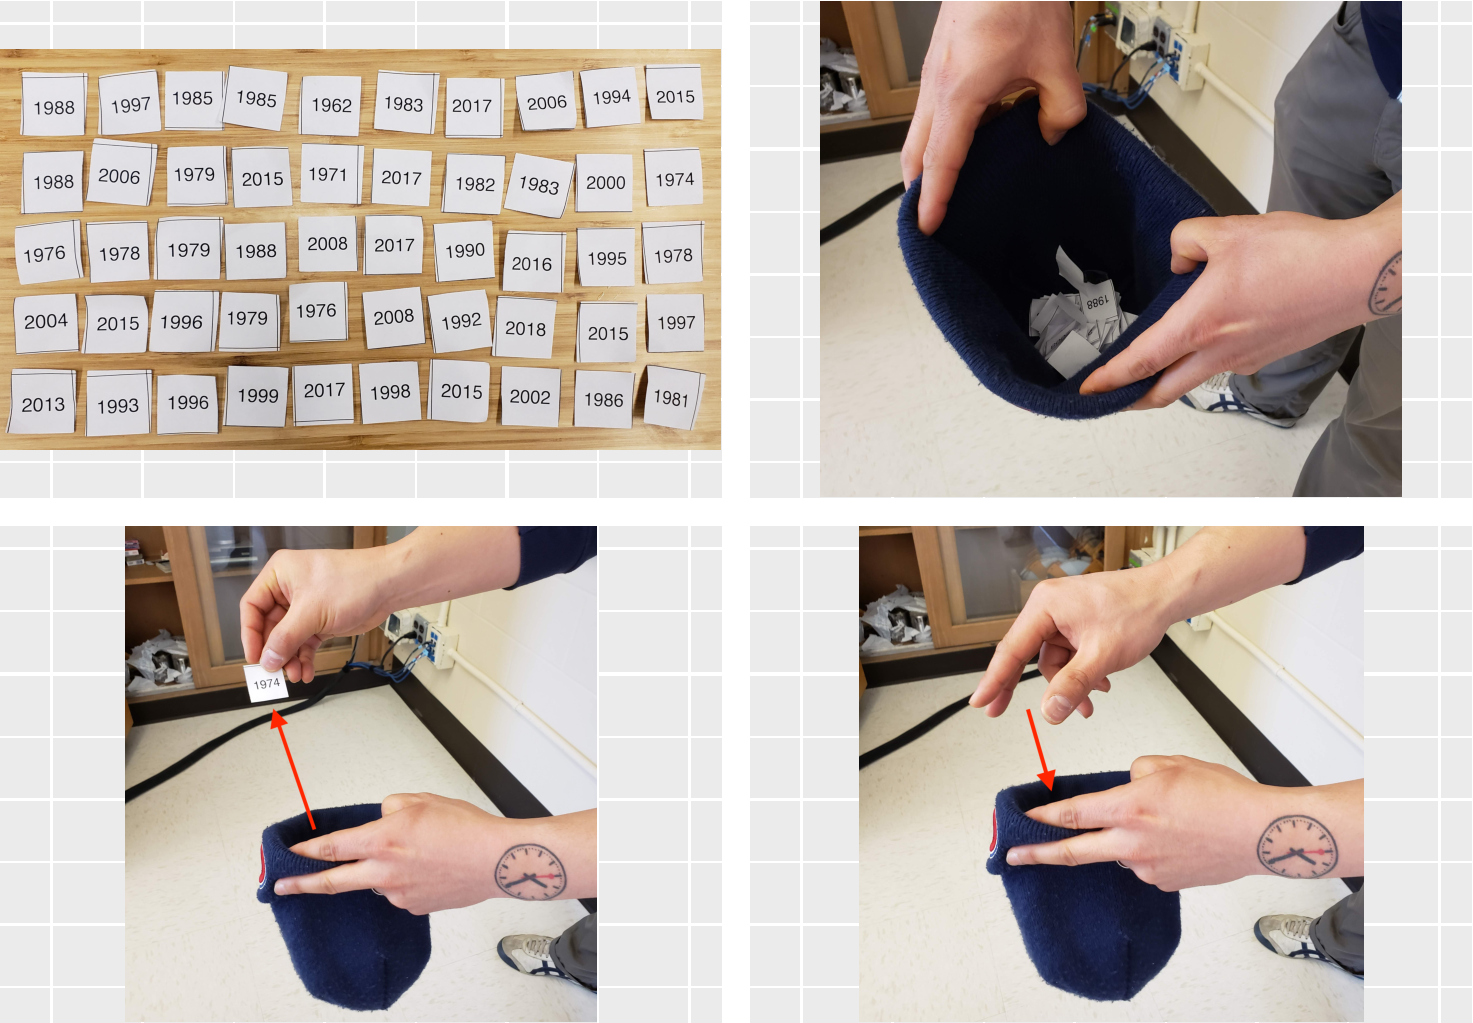
\includegraphics[width=0.8\linewidth,height=0.5\textheight]{Week5_Lect_files/figure-beamer/unnamed-chunk-8-1} \end{center}
\normalsize
\end{frame}

\begin{frame}[fragile]{Exploratory data analysis}
\protect\hypertarget{exploratory-data-analysis-7}{}
\normalsize

\begin{Shaded}
\begin{Highlighting}[]
\NormalTok{lifeExp\_by\_continent }\OtherTok{\textless{}{-}}\NormalTok{ gapminder2007 }\SpecialCharTok{\%\textgreater{}\%}
  \FunctionTok{group\_by}\NormalTok{(continent) }\SpecialCharTok{\%\textgreater{}\%}
  \FunctionTok{summarize}\NormalTok{(}\AttributeTok{median =} \FunctionTok{median}\NormalTok{(lifeExp), }
            \AttributeTok{mean =} \FunctionTok{mean}\NormalTok{(lifeExp)) }\SpecialCharTok{\%\textgreater{}\%} 
  \FunctionTok{mutate}\NormalTok{(}\StringTok{\textasciigrave{}}\AttributeTok{Difference versus Africa}\StringTok{\textasciigrave{}} \OtherTok{=}\NormalTok{ mean }\SpecialCharTok{{-}}\NormalTok{ mean[}\DecValTok{1}\NormalTok{])}
\NormalTok{knitr}\SpecialCharTok{::}\FunctionTok{kable}\NormalTok{(lifeExp\_by\_continent)}
\end{Highlighting}
\end{Shaded}

\begin{longtable}[]{@{}lrrr@{}}
\toprule\noalign{}
continent & median & mean & Difference versus Africa \\
\midrule\noalign{}
\endhead
Africa & 52.9265 & 54.80604 & 0.00000 \\
Americas & 72.8990 & 73.60812 & 18.80208 \\
Asia & 72.3960 & 70.72848 & 15.92245 \\
Europe & 78.6085 & 77.64860 & 22.84256 \\
Oceania & 80.7195 & 80.71950 & 25.91346 \\
\bottomrule\noalign{}
\end{longtable}

\normalsize
\end{frame}

\begin{frame}[fragile]{Linear regression}
\protect\hypertarget{linear-regression}{}
In our life expectancy example, we now instead have a
\textbf{categorical} explanatory variable \texttt{continent}:

\tiny

\begin{Shaded}
\begin{Highlighting}[]
\NormalTok{lifeExp\_model }\OtherTok{\textless{}{-}} \FunctionTok{lm}\NormalTok{(lifeExp }\SpecialCharTok{\textasciitilde{}}\NormalTok{ continent, }\AttributeTok{data =}\NormalTok{ gapminder2007)}
\NormalTok{knitr}\SpecialCharTok{::}\FunctionTok{kable}\NormalTok{(}\FunctionTok{get\_regression\_table}\NormalTok{(lifeExp\_model))}
\end{Highlighting}
\end{Shaded}

\begin{longtable}[]{@{}
  >{\raggedright\arraybackslash}p{(\columnwidth - 12\tabcolsep) * \real{0.2667}}
  >{\raggedleft\arraybackslash}p{(\columnwidth - 12\tabcolsep) * \real{0.1200}}
  >{\raggedleft\arraybackslash}p{(\columnwidth - 12\tabcolsep) * \real{0.1333}}
  >{\raggedleft\arraybackslash}p{(\columnwidth - 12\tabcolsep) * \real{0.1333}}
  >{\raggedleft\arraybackslash}p{(\columnwidth - 12\tabcolsep) * \real{0.1067}}
  >{\raggedleft\arraybackslash}p{(\columnwidth - 12\tabcolsep) * \real{0.1200}}
  >{\raggedleft\arraybackslash}p{(\columnwidth - 12\tabcolsep) * \real{0.1200}}@{}}
\toprule\noalign{}
\begin{minipage}[b]{\linewidth}\raggedright
term
\end{minipage} & \begin{minipage}[b]{\linewidth}\raggedleft
estimate
\end{minipage} & \begin{minipage}[b]{\linewidth}\raggedleft
std\_error
\end{minipage} & \begin{minipage}[b]{\linewidth}\raggedleft
statistic
\end{minipage} & \begin{minipage}[b]{\linewidth}\raggedleft
p\_value
\end{minipage} & \begin{minipage}[b]{\linewidth}\raggedleft
lower\_ci
\end{minipage} & \begin{minipage}[b]{\linewidth}\raggedleft
upper\_ci
\end{minipage} \\
\midrule\noalign{}
\endhead
intercept & 54.806 & 1.025 & 53.446 & 0 & 52.778 & 56.834 \\
continent: Americas & 18.802 & 1.800 & 10.448 & 0 & 15.243 & 22.361 \\
continent: Asia & 15.922 & 1.646 & 9.675 & 0 & 12.668 & 19.177 \\
continent: Europe & 22.843 & 1.695 & 13.474 & 0 & 19.490 & 26.195 \\
continent: Oceania & 25.913 & 5.328 & 4.863 & 0 & 15.377 & 36.450 \\
\bottomrule\noalign{}
\end{longtable}

\normalsize

Our model will not yield a ``best-fitting'' regression line like when
the \(x\) is continuous, but rather offsets relative to a baseline for
comparison.
\end{frame}

\begin{frame}[fragile]{Linear regression}
\protect\hypertarget{linear-regression-1}{}
Let's break the 5 estimates down one-by-one:

\begin{itemize}
\item
  \texttt{intercept} corresponds to the mean life expectancy of
  countries in Africa of 54.8 years.
\item
  \texttt{continent:\ Americas} corresponds to countries in the Americas
  and the value +18.8 is the same difference in mean life expectancy
  relative to Africa we displayed earlier. In other words, the mean life
  expectancy of countries in the Americas is \(54.8+18.8=73.6\).
\item
  \texttt{continent:\ Asia} the mean life expectancy of countries in
  Asia is \(54.8+ 15.9=70.7\).
\item
  \texttt{continent:\ Europe} the mean life expectancy of countries in
  Europe is \(54.8+22.8=77.6\).
\item
  \texttt{continent:\ Oceania} the mean life expectancy of countries in
  Oceania is \(54.8+25.9=80.7\).
\end{itemize}
\end{frame}

\begin{frame}[fragile]{Linear regression}
\protect\hypertarget{linear-regression-2}{}
We can change the baseline group to be another continent. In what
follows the baseline is changed to be \texttt{Americas} instead of
\texttt{Africa}.

\tiny

\begin{Shaded}
\begin{Highlighting}[]
\NormalTok{gapminder2007}\SpecialCharTok{$}\NormalTok{continent }\OtherTok{\textless{}{-}} \FunctionTok{relevel}\NormalTok{(gapminder2007}\SpecialCharTok{$}\NormalTok{continent, }\AttributeTok{ref=}\StringTok{\textquotesingle{}Americas\textquotesingle{}}\NormalTok{)}
\NormalTok{lifeExp\_model1 }\OtherTok{\textless{}{-}} \FunctionTok{lm}\NormalTok{(lifeExp }\SpecialCharTok{\textasciitilde{}}\NormalTok{ continent, }\AttributeTok{data =}\NormalTok{ gapminder2007)}
\NormalTok{knitr}\SpecialCharTok{::}\FunctionTok{kable}\NormalTok{(}\FunctionTok{get\_regression\_table}\NormalTok{(lifeExp\_model1))}
\end{Highlighting}
\end{Shaded}

\begin{longtable}[]{@{}
  >{\raggedright\arraybackslash}p{(\columnwidth - 12\tabcolsep) * \real{0.2568}}
  >{\raggedleft\arraybackslash}p{(\columnwidth - 12\tabcolsep) * \real{0.1216}}
  >{\raggedleft\arraybackslash}p{(\columnwidth - 12\tabcolsep) * \real{0.1351}}
  >{\raggedleft\arraybackslash}p{(\columnwidth - 12\tabcolsep) * \real{0.1351}}
  >{\raggedleft\arraybackslash}p{(\columnwidth - 12\tabcolsep) * \real{0.1081}}
  >{\raggedleft\arraybackslash}p{(\columnwidth - 12\tabcolsep) * \real{0.1216}}
  >{\raggedleft\arraybackslash}p{(\columnwidth - 12\tabcolsep) * \real{0.1216}}@{}}
\toprule\noalign{}
\begin{minipage}[b]{\linewidth}\raggedright
term
\end{minipage} & \begin{minipage}[b]{\linewidth}\raggedleft
estimate
\end{minipage} & \begin{minipage}[b]{\linewidth}\raggedleft
std\_error
\end{minipage} & \begin{minipage}[b]{\linewidth}\raggedleft
statistic
\end{minipage} & \begin{minipage}[b]{\linewidth}\raggedleft
p\_value
\end{minipage} & \begin{minipage}[b]{\linewidth}\raggedleft
lower\_ci
\end{minipage} & \begin{minipage}[b]{\linewidth}\raggedleft
upper\_ci
\end{minipage} \\
\midrule\noalign{}
\endhead
intercept & 73.608 & 1.479 & 49.772 & 0.000 & 70.684 & 76.533 \\
continent: Africa & -18.802 & 1.800 & -10.448 & 0.000 & -22.361 &
-15.243 \\
continent: Asia & -2.880 & 1.961 & -1.469 & 0.144 & -6.757 & 0.997 \\
continent: Europe & 4.040 & 2.002 & 2.018 & 0.046 & 0.081 & 8.000 \\
continent: Oceania & 7.111 & 5.434 & 1.309 & 0.193 & -3.634 & 17.857 \\
\bottomrule\noalign{}
\end{longtable}

\normalsize
\end{frame}

\begin{frame}[fragile]{Linear regression}
\protect\hypertarget{linear-regression-3}{}
The equation for our fitted values for model (\texttt{lifeExp\_model})
is written as:

\[\begin{array}{ll}
\hat{y}&=\widehat{\text{life exp}}=b_0+b_{\text{Amer}}\cdot1_{\text{Amer}}(x)+b_{\text{Asia}}\cdot1_{\text{Asia}}(x)\\
&+b_{\text{Euro}}\cdot1_{\text{Euro}}(x)+b_{\text{Ocean}}\cdot1_{\text{Ocean}}(x)\\
&=54.8+18.8\cdot1_{\text{Amer}}(x)+15.9\cdot 1_{\text{Asia}}(x)\\
&+22.8\cdot 1_{\text{Euro}}(x)+25.9\cdot 1_{\text{Ocean}}(x).
\end{array}\]

where for example:
\[1_{\text{Amer}}(x)=\left\{\begin{array}{ll} 1 & \text{if country } x \text{ is in the Americas }\\
0 & \text{if otherwise} \end{array}\right.\]
\end{frame}

\begin{frame}{Linear regression}
\protect\hypertarget{linear-regression-4}{}
Let's put this all together and compute the fitted value
\(\hat{y}=\widehat{\text{life exp}}\) for a country in Africa.

\begin{itemize}
\tightlist
\item
  Since the country is in Africa, all four indicator functions
  \(1_{\text{Euro}}(x)=1_{\text{Amer}}(x)=1_{\text{Asia}}(x)=1_{\text{Ocean}}(x)=0\).
\end{itemize}

\[\begin{array}{ll}
\hat{y}=\widehat{\text{life exp}}&=54.8+18.8\cdot1_{\text{Amer}}(x)+15.9\cdot 1_{\text{Asia}}(x)\\
&+22.8\cdot 1_{\text{Euro}}(x)+25.9\cdot 1_{\text{Ocean}}(x).\\
&=54.8+18.8\cdot0+15.9\cdot 0+22.8\cdot 0+25.9\cdot 0\\
&=54.8
\end{array}\]
\end{frame}

\begin{frame}{Linear regression}
\protect\hypertarget{linear-regression-5}{}
For a country in in the Americas, in this case, only the indicator
function \(1_{\text{Amer}}(x)=1\).

\[\begin{array}{ll}
\hat{y}=\widehat{\text{life exp}}&=54.8+18.8\cdot1_{\text{Amer}}(x)+15.9\cdot 1_{\text{Asia}}(x)\\
&+22.8\cdot 1_{\text{Euro}}(x)+25.9\cdot 1_{\text{Ocean}}(x).\\
&=54.8+18.8\cdot1+15.9\cdot 0+22.8\cdot 0+25.9\cdot 0\\
&=73.6
\end{array}\]

In general, if we fit a linear regression model using a categorical
explanatory variable \(x\) that has \(k\) possible categories, the
regression table will return an intercept and \(k-1\) offsets.
\end{frame}

\begin{frame}[fragile]{Observed/fitted values and residuals}
\protect\hypertarget{observedfitted-values-and-residuals}{}
\normalsize

\begin{Shaded}
\begin{Highlighting}[]
\NormalTok{regression\_points }\OtherTok{\textless{}{-}} \FunctionTok{get\_regression\_points}\NormalTok{(lifeExp\_model, }
                                           \AttributeTok{ID =} \StringTok{"country"}\NormalTok{) }
\NormalTok{knitr}\SpecialCharTok{::}\FunctionTok{kable}\NormalTok{(regression\_points }\SpecialCharTok{\%\textgreater{}\%} \FunctionTok{head}\NormalTok{(}\AttributeTok{n =} \DecValTok{9}\NormalTok{))}
\end{Highlighting}
\end{Shaded}

\begin{longtable}[]{@{}lrlrr@{}}
\toprule\noalign{}
country & lifeExp & continent & lifeExp\_hat & residual \\
\midrule\noalign{}
\endhead
Afghanistan & 43.828 & Asia & 70.728 & -26.900 \\
Albania & 76.423 & Europe & 77.649 & -1.226 \\
Algeria & 72.301 & Africa & 54.806 & 17.495 \\
Angola & 42.731 & Africa & 54.806 & -12.075 \\
Argentina & 75.320 & Americas & 73.608 & 1.712 \\
Australia & 81.235 & Oceania & 80.720 & 0.516 \\
Austria & 79.829 & Europe & 77.649 & 2.180 \\
Bahrain & 75.635 & Asia & 70.728 & 4.907 \\
Bangladesh & 64.062 & Asia & 70.728 & -6.666 \\
\bottomrule\noalign{}
\end{longtable}

\normalsize
\end{frame}

\hypertarget{multiple-regression}{%
\section{Multiple Regression}\label{multiple-regression}}

\begin{frame}{Multiple Regression}
\protect\hypertarget{multiple-regression-1}{}
In the previous chapter, we introduced ideas related to modeling for
\textbf{explanation.}

\begin{itemize}
\item
  In particular that the goal of modeling is to make explicit the
  relationship between some outcome variable \(y\) and some explanatory
  variable \(x\).
\item
  We focused on linear regression, where we only considered one
  explanatory \(x\) variable that is either numeric or categorical.
\item
  Now, we we'll start considering models that include more than one
  explanatory variable \(x\).

  \begin{itemize}
  \tightlist
  \item
    NOTE: the interpretation of the associated effect of any one
    explanatory variable must be made in conjunction with the other
    explanatory variables included in your model.
  \end{itemize}
\end{itemize}
\end{frame}

\begin{frame}[fragile]{Needed packages}
\protect\hypertarget{needed-packages-1}{}
Let's load all the packages needed for this chapter.

\normalsize

\begin{Shaded}
\begin{Highlighting}[]
\FunctionTok{library}\NormalTok{(tidyverse) }
\FunctionTok{library}\NormalTok{(moderndive)}
\FunctionTok{library}\NormalTok{(skimr)}
\FunctionTok{library}\NormalTok{(ISLR)}
\end{Highlighting}
\end{Shaded}

\normalsize
\end{frame}

\begin{frame}[fragile]{One numerical and one categorical explanatory
variable}
\protect\hypertarget{one-numerical-and-one-categorical-explanatory-variable}{}
Let's revisit the instructor evaluation data we introduced earlier.

\begin{itemize}
\item
  We studied the relationship between teaching evaluation scores as
  given by students and ``beauty'' scores.

  \begin{itemize}
  \tightlist
  \item
    The variable teaching score was the numerical outcome variable
    \(y\), and the variable ``beauty'' score (\texttt{bty\_avg}) was the
    numerical explanatory \(x\) variable.
  \end{itemize}
\item
  In this section, we are going to consider a different model

  \begin{itemize}
  \tightlist
  \item
    Our outcome variable will still be teaching score, but
  \item
    we'll now include two different explanatory variables: \texttt{age}
    and \texttt{gender}.
  \item
    Could it be that instructors who are older receive better teaching
    evaluations from students?
  \item
    Or could it instead be that younger instructors receive better
    evaluations?
  \item
    Are there differences in evaluations given by students for
    instructors of different genders?
  \end{itemize}
\end{itemize}
\end{frame}

\begin{frame}[fragile]{Exploratory data analysis}
\protect\hypertarget{exploratory-data-analysis-8}{}
Let's \texttt{select()} only the subset of the variables we'll consider
in this chapter.

\normalsize

\begin{Shaded}
\begin{Highlighting}[]
\NormalTok{evals\_ch6 }\OtherTok{\textless{}{-}}\NormalTok{ evals }\SpecialCharTok{\%\textgreater{}\%}
  \FunctionTok{select}\NormalTok{(ID, score, age, gender)}
\end{Highlighting}
\end{Shaded}

\normalsize

Recall the three common steps in an exploratory data analysis:

\begin{enumerate}
\tightlist
\item
  Looking at the raw data values.
\item
  Computing summary statistics.
\item
  Creating data visualizations.
\end{enumerate}
\end{frame}

\begin{frame}[fragile]{Exploratory data analysis}
\protect\hypertarget{exploratory-data-analysis-9}{}
Let's first look at the raw data values.

\small

\begin{Shaded}
\begin{Highlighting}[]
\FunctionTok{glimpse}\NormalTok{(evals\_ch6)}
\end{Highlighting}
\end{Shaded}

\begin{verbatim}
Rows: 463
Columns: 4
$ ID     <int> 1, 2, 3, 4, 5, 6, 7, 8, 9, 10, 11, 12, 13, 14, 15, 16, 17, 18, ~
$ score  <dbl> 4.7, 4.1, 3.9, 4.8, 4.6, 4.3, 2.8, 4.1, 3.4, 4.5, 3.8, 4.5, 4.6~
$ age    <int> 36, 36, 36, 36, 59, 59, 59, 51, 51, 40, 40, 40, 40, 40, 40, 40,~
$ gender <fct> female, female, female, female, male, male, male, male, male, f~
\end{verbatim}

\begin{Shaded}
\begin{Highlighting}[]
\CommentTok{\# Or}
\NormalTok{evals\_ch6 }\SpecialCharTok{\%\textgreater{}\%} 
  \FunctionTok{sample\_n}\NormalTok{(}\AttributeTok{size =} \DecValTok{2}\NormalTok{)}
\end{Highlighting}
\end{Shaded}

\begin{verbatim}
# A tibble: 2 x 4
     ID score   age gender
  <int> <dbl> <int> <fct> 
1   434   2.8    62 male  
2   208   4.4    62 male  
\end{verbatim}

\normalsize
\end{frame}

\begin{frame}[fragile]{Exploratory data analysis}
\protect\hypertarget{exploratory-data-analysis-10}{}
\normalsize

\begin{Shaded}
\begin{Highlighting}[]
\NormalTok{evals\_ch6 }\SpecialCharTok{\%\textgreater{}\%} 
  \FunctionTok{select}\NormalTok{(score, age, gender) }\SpecialCharTok{\%\textgreater{}\%} 
  \FunctionTok{skim}\NormalTok{()}
\end{Highlighting}
\end{Shaded}

\normalsize

\begin{Shaded}
\begin{Highlighting}[]
\CommentTok{\# Or}
\NormalTok{evals\_ch6 }\SpecialCharTok{\%\textgreater{}\%} 
  \FunctionTok{select}\NormalTok{(score, age, gender) }\SpecialCharTok{\%\textgreater{}\%} 
  \FunctionTok{summary}\NormalTok{()}
\end{Highlighting}
\end{Shaded}

\begin{verbatim}
     score            age           gender   
 Min.   :2.300   Min.   :29.00   female:195  
 1st Qu.:3.800   1st Qu.:42.00   male  :268  
 Median :4.300   Median :48.00               
 Mean   :4.175   Mean   :48.37               
 3rd Qu.:4.600   3rd Qu.:57.00               
 Max.   :5.000   Max.   :73.00               
\end{verbatim}
\end{frame}

\begin{frame}[fragile]{Exploratory data analysis}
\protect\hypertarget{exploratory-data-analysis-11}{}
Let's compute the correlation coefficient between our two numerical
variables: \texttt{score} and \texttt{age}:

\small

\begin{Shaded}
\begin{Highlighting}[]
\NormalTok{evals\_ch6 }\SpecialCharTok{\%\textgreater{}\%} 
  \FunctionTok{summarize}\NormalTok{(}\AttributeTok{r =} \FunctionTok{cor}\NormalTok{(score, age))}
\end{Highlighting}
\end{Shaded}

\begin{verbatim}
# A tibble: 1 x 1
       r
   <dbl>
1 -0.107
\end{verbatim}

\begin{Shaded}
\begin{Highlighting}[]
\CommentTok{\# or using the get\_correlation wrapper}
\CommentTok{\# from moderndive}
\NormalTok{evals\_ch6 }\SpecialCharTok{\%\textgreater{}\%} 
  \FunctionTok{get\_correlation}\NormalTok{(score }\SpecialCharTok{\textasciitilde{}}\NormalTok{ age)}
\end{Highlighting}
\end{Shaded}

\begin{verbatim}
# A tibble: 1 x 1
     cor
   <dbl>
1 -0.107
\end{verbatim}

\normalsize
\end{frame}

\begin{frame}[fragile]{Exploratory data analysis}
\protect\hypertarget{exploratory-data-analysis-12}{}
\normalsize

\begin{Shaded}
\begin{Highlighting}[]
\FunctionTok{ggplot}\NormalTok{(evals\_ch6, }\FunctionTok{aes}\NormalTok{(}\AttributeTok{x =}\NormalTok{ age, }\AttributeTok{y =}\NormalTok{ score, }\AttributeTok{color =}\NormalTok{ gender)) }\SpecialCharTok{+}
  \FunctionTok{geom\_point}\NormalTok{() }\SpecialCharTok{+}
  \FunctionTok{labs}\NormalTok{(}\AttributeTok{x =} \StringTok{"Age"}\NormalTok{, }\AttributeTok{y =} \StringTok{"Teaching Score"}\NormalTok{, }\AttributeTok{color =} \StringTok{"Gender"}\NormalTok{,}
       \AttributeTok{title =} \StringTok{"Interaction Model"}\NormalTok{) }\SpecialCharTok{+}
  \FunctionTok{geom\_smooth}\NormalTok{(}\AttributeTok{method =} \StringTok{"lm"}\NormalTok{, }\AttributeTok{se =} \ConstantTok{FALSE}\NormalTok{) }\SpecialCharTok{+} 
  \FunctionTok{theme\_bw}\NormalTok{() }\OtherTok{{-}\textgreater{}}\NormalTok{ int\_mod}
\NormalTok{int\_mod}
\end{Highlighting}
\end{Shaded}

\normalsize
\end{frame}

\begin{frame}{Exploratory data analysis}
\protect\hypertarget{exploratory-data-analysis-13}{}
\normalsize
\begin{figure}

{\centering \includegraphics[width=0.9\linewidth,height=0.9\textheight]{Week5_Lect_files/figure-beamer/interaction-1} 

}

\caption{Interaction Model}\label{fig:interaction}
\end{figure}
\normalsize
\end{frame}

\begin{frame}[fragile]{Interaction model}
\protect\hypertarget{interaction-model}{}
\begin{itemize}
\item
  Let's now quantify the relationship of our outcome variable \(y\) and
  the two explanatory variables using one type of multiple regression
  model known as an \textbf{interaction model}.
\item
  Going back to our multiple regression model for teaching
  \texttt{score} using \texttt{age} and \texttt{gender} in the figure
  above, we generate the regression table using the same two-step
  approach.

  \begin{enumerate}
  \tightlist
  \item
    First, ``fit'' a model using the \texttt{lm()} (linear model)
    function of the form
    \texttt{y\ \textasciitilde{}x1\ +\ x2\ +\ x1:x2} which is the same
    as \texttt{y\ \textasciitilde{}\ x1*x2} in R's modeling notation.
  \item
    Second, apply \texttt{get\_regression\_table()} or
    \texttt{summary()} to the linear model object created in 1.
  \end{enumerate}
\end{itemize}
\end{frame}

\begin{frame}[fragile]{Interaction model}
\protect\hypertarget{interaction-model-1}{}
\small

\begin{Shaded}
\begin{Highlighting}[]
\CommentTok{\# Fit regression model:}
\NormalTok{score\_model\_interaction }\OtherTok{\textless{}{-}} \FunctionTok{lm}\NormalTok{(score }\SpecialCharTok{\textasciitilde{}}\NormalTok{ age }\SpecialCharTok{+}\NormalTok{ gender }\SpecialCharTok{+}\NormalTok{ age}\SpecialCharTok{:}\NormalTok{gender, }
                              \AttributeTok{data =}\NormalTok{ evals\_ch6)}
\CommentTok{\# Get regression table:}
\NormalTok{knitr}\SpecialCharTok{::}\FunctionTok{kable}\NormalTok{(}\FunctionTok{get\_regression\_table}\NormalTok{(score\_model\_interaction))}
\end{Highlighting}
\end{Shaded}

\begin{longtable}[]{@{}
  >{\raggedright\arraybackslash}p{(\columnwidth - 12\tabcolsep) * \real{0.2143}}
  >{\raggedleft\arraybackslash}p{(\columnwidth - 12\tabcolsep) * \real{0.1286}}
  >{\raggedleft\arraybackslash}p{(\columnwidth - 12\tabcolsep) * \real{0.1429}}
  >{\raggedleft\arraybackslash}p{(\columnwidth - 12\tabcolsep) * \real{0.1429}}
  >{\raggedleft\arraybackslash}p{(\columnwidth - 12\tabcolsep) * \real{0.1143}}
  >{\raggedleft\arraybackslash}p{(\columnwidth - 12\tabcolsep) * \real{0.1286}}
  >{\raggedleft\arraybackslash}p{(\columnwidth - 12\tabcolsep) * \real{0.1286}}@{}}
\toprule\noalign{}
\begin{minipage}[b]{\linewidth}\raggedright
term
\end{minipage} & \begin{minipage}[b]{\linewidth}\raggedleft
estimate
\end{minipage} & \begin{minipage}[b]{\linewidth}\raggedleft
std\_error
\end{minipage} & \begin{minipage}[b]{\linewidth}\raggedleft
statistic
\end{minipage} & \begin{minipage}[b]{\linewidth}\raggedleft
p\_value
\end{minipage} & \begin{minipage}[b]{\linewidth}\raggedleft
lower\_ci
\end{minipage} & \begin{minipage}[b]{\linewidth}\raggedleft
upper\_ci
\end{minipage} \\
\midrule\noalign{}
\endhead
intercept & 4.883 & 0.205 & 23.795 & 0.000 & 4.480 & 5.286 \\
age & -0.018 & 0.004 & -3.919 & 0.000 & -0.026 & -0.009 \\
gender: male & -0.446 & 0.265 & -1.681 & 0.094 & -0.968 & 0.076 \\
age:gendermale & 0.014 & 0.006 & 2.446 & 0.015 & 0.003 & 0.024 \\
\bottomrule\noalign{}
\end{longtable}

\normalsize
\end{frame}

\begin{frame}[fragile]{Interaction model}
\protect\hypertarget{interaction-model-2}{}
Female instructors are the ``baseline for comparison'' group.

\begin{itemize}
\tightlist
\item
  The estimate for \texttt{intercept} is the intercept for only the
  \texttt{female} instructors.
\item
  The estimate for \texttt{age} is the slope for age for only the female
  instructors.
\item
  Thus, the red regression line in Figure 1 has an intercept of 4.883
  and slope for \texttt{age} of -0.018.
\item
  Note: The intercept has no practical interpretation since instructors
  can not have a \textbf{zero} age.
\end{itemize}
\end{frame}

\begin{frame}[fragile]{Interaction model}
\protect\hypertarget{interaction-model-3}{}
What about the intercept and slope for age of the male instructors in
the blue line of Figure 1?

\begin{itemize}
\item
  The value for \texttt{gender:\ male} that appears in the Table
  (-0.446) is not the intercept for the male instructors but rather the
  offset in intercept for male instructors relative to female
  instructors.

  \begin{itemize}
  \tightlist
  \item
    The intercept for the male instructors is
    \texttt{intercept\ +\ gender:male} =
    \(4.883 + (-0.446) = 4.883 - 0.446 = 4.437\).
  \end{itemize}
\item
  Similarly, \texttt{age:gendermale} = 0.014 is not the slope for age
  for the male instructors, but rather the offset in slope for the male
  instructors.

  \begin{itemize}
  \tightlist
  \item
    Therefore, the slope for \texttt{age} for the male instructors is
    \texttt{age\ +\ age:gendermale} =\(-0.018 + 0.014 = -0.004\).
  \end{itemize}
\end{itemize}
\end{frame}

\begin{frame}[fragile]{Interaction model}
\protect\hypertarget{interaction-model-4}{}
\begin{center}\includegraphics[width=0.6\linewidth,height=0.3\textheight]{week5_2} \end{center}

\begin{itemize}
\item
  Since the slope for age for the female instructors was -0.018, it
  means that on average, a female instructor who is a year older would
  have a teaching score that is 0.018 units \textbf{lower}.
\item
  For the male instructors, the associated decrease in score is 0.004
  units.
\item
  While both slopes for \texttt{age} were negative, the slope for
  \texttt{age} for the female instructors is \textbf{larger} in
  magnitude.
\end{itemize}
\end{frame}

\begin{frame}{Interaction model: Prediction}
\protect\hypertarget{interaction-model-prediction}{}
Let's now write the equation for our regression lines, which we can use
to compute our fitted values

\[\begin{array}{ll}
\hat{y}&=\widehat{\text{score}}=b_0+b_{\text{age}}\cdot \text{age}+b_{\text{male}}\cdot 1_{\text{is male}}(x)+b_{\text{age:gender}}\cdot \text{age}\cdot 1_{\text{is male}}(x)\\
&=4.883-0.018\cdot \text{age}-0.446\cdot 1_{\text{is male}}(x)+0.014\cdot \text{age}\cdot1_{\text{is male}}(x).
\end{array}\]

where:

\[1_{\text{is male}}(x)=\left\{\begin{array}{ll} 1 & \text{if instructor } x \text{ is male }\\
0 & \text{otherwise} \end{array}\right.\]
\end{frame}

\begin{frame}{Interaction model: Prediction}
\protect\hypertarget{interaction-model-prediction-1}{}
Let's put this all together and compute the fitted
value\(\hat{y}=\widehat{\text{score}}\) for female instructors.

\begin{itemize}
\tightlist
\item
  Since for female instructors \(1_{\text{is male}}(x)=0\).
\end{itemize}

\[\begin{array}{ll}
\hat{y}=\widehat{\text{score}}&=4.883-0.018\cdot \text{age}-0.446\cdot 0+0.014\cdot \text{age}\cdot 0.\\
&=4.883-0.018\cdot \text{age}
\end{array}\]

\begin{itemize}
\tightlist
\item
  For male instructors \(1_{\text{is male}}(x)=1\).
\end{itemize}

\[\begin{array}{ll}
\hat{y}=\widehat{\text{score}}&=4.883-0.018\cdot \text{age}-0.446\cdot 1+0.014\cdot \text{age}\cdot 1.\\
&=(4.883-0.446)+(-0.018+0.014)\cdot \text{age}\\
&=4.437-0.004\cdot \text{age}
\end{array}\]
\end{frame}

\begin{frame}{Interaction model: Explanation}
\protect\hypertarget{interaction-model-explanation}{}
\begin{itemize}
\item
  The term \(b_{\text{age:gender}}\) in the equation for the fitted
  value \(\hat{y}=\widehat{\text{score}}\) is what's known in
  statistical modeling as an \textbf{interaction effect}.
\item
  We say there is an interaction effect if the associated effect of one
  variable depends on the value of another variable.

  \begin{itemize}
  \tightlist
  \item
    Here, the associated effect of the variable age depends on the value
    of the other variable gender.
  \item
    The difference in slopes for age of +0.014 of male instructors
    relative to female instructors shows this.
  \end{itemize}
\end{itemize}
\end{frame}

\begin{frame}[fragile]{Parallel slopes model}
\protect\hypertarget{parallel-slopes-model}{}
With one numerical and one categorical explanatory variable, another
type of model we can use is known as a \textbf{parallel slopes} model.

\begin{itemize}
\tightlist
\item
  Unlike interaction models, parallel slopes models still allow for
  different intercepts but force all lines to have the same slope.
\end{itemize}

\normalsize

\begin{Shaded}
\begin{Highlighting}[]
\FunctionTok{ggplot}\NormalTok{(evals\_ch6, }\FunctionTok{aes}\NormalTok{(}\AttributeTok{x =}\NormalTok{ age, }\AttributeTok{y =}\NormalTok{ score, }\AttributeTok{color =}\NormalTok{ gender)) }\SpecialCharTok{+}
  \FunctionTok{geom\_point}\NormalTok{() }\SpecialCharTok{+}
  \FunctionTok{labs}\NormalTok{(}\AttributeTok{x =} \StringTok{"Age"}\NormalTok{, }\AttributeTok{y =} \StringTok{"Teaching Score"}\NormalTok{, }\AttributeTok{color =} \StringTok{"Gender"}\NormalTok{,}
       \AttributeTok{title =} \StringTok{"Parallel Slopes Model"}\NormalTok{) }\SpecialCharTok{+}
  \FunctionTok{geom\_parallel\_slopes}\NormalTok{(}\AttributeTok{se =} \ConstantTok{FALSE}\NormalTok{) }\SpecialCharTok{+} 
  \FunctionTok{theme\_bw}\NormalTok{() }\OtherTok{{-}\textgreater{}}\NormalTok{ ps\_mod}
\NormalTok{ps\_mod}
\end{Highlighting}
\end{Shaded}

\normalsize
\end{frame}

\begin{frame}{Parallel slopes model}
\protect\hypertarget{parallel-slopes-model-1}{}
\normalsize

\begin{center}\includegraphics[width=0.9\linewidth,height=0.9\textheight]{Week5_Lect_files/figure-beamer/unnamed-chunk-23-1} \end{center}
\normalsize
\end{frame}

\begin{frame}[fragile]{Parallel slopes model}
\protect\hypertarget{parallel-slopes-model-2}{}
\small

\begin{Shaded}
\begin{Highlighting}[]
\CommentTok{\# Fit regression model:}
\NormalTok{score\_model\_parallel\_slopes }\OtherTok{\textless{}{-}} \FunctionTok{lm}\NormalTok{(score }\SpecialCharTok{\textasciitilde{}}\NormalTok{ age }\SpecialCharTok{+}\NormalTok{ gender, }
                                  \AttributeTok{data =}\NormalTok{ evals\_ch6)}
\CommentTok{\# Get regression table:}
\NormalTok{knitr}\SpecialCharTok{::}\FunctionTok{kable}\NormalTok{(}\FunctionTok{get\_regression\_table}\NormalTok{(score\_model\_parallel\_slopes))}
\end{Highlighting}
\end{Shaded}

\begin{longtable}[]{@{}
  >{\raggedright\arraybackslash}p{(\columnwidth - 12\tabcolsep) * \real{0.1912}}
  >{\raggedleft\arraybackslash}p{(\columnwidth - 12\tabcolsep) * \real{0.1324}}
  >{\raggedleft\arraybackslash}p{(\columnwidth - 12\tabcolsep) * \real{0.1471}}
  >{\raggedleft\arraybackslash}p{(\columnwidth - 12\tabcolsep) * \real{0.1471}}
  >{\raggedleft\arraybackslash}p{(\columnwidth - 12\tabcolsep) * \real{0.1176}}
  >{\raggedleft\arraybackslash}p{(\columnwidth - 12\tabcolsep) * \real{0.1324}}
  >{\raggedleft\arraybackslash}p{(\columnwidth - 12\tabcolsep) * \real{0.1324}}@{}}
\toprule\noalign{}
\begin{minipage}[b]{\linewidth}\raggedright
term
\end{minipage} & \begin{minipage}[b]{\linewidth}\raggedleft
estimate
\end{minipage} & \begin{minipage}[b]{\linewidth}\raggedleft
std\_error
\end{minipage} & \begin{minipage}[b]{\linewidth}\raggedleft
statistic
\end{minipage} & \begin{minipage}[b]{\linewidth}\raggedleft
p\_value
\end{minipage} & \begin{minipage}[b]{\linewidth}\raggedleft
lower\_ci
\end{minipage} & \begin{minipage}[b]{\linewidth}\raggedleft
upper\_ci
\end{minipage} \\
\midrule\noalign{}
\endhead
intercept & 4.484 & 0.125 & 35.792 & 0.000 & 4.238 & 4.730 \\
age & -0.009 & 0.003 & -3.280 & 0.001 & -0.014 & -0.003 \\
gender: male & 0.191 & 0.052 & 3.632 & 0.000 & 0.087 & 0.294 \\
\bottomrule\noalign{}
\end{longtable}

\normalsize

\begin{center}\includegraphics[width=0.6\linewidth,height=0.2\textheight]{week5_3} \end{center}
\end{frame}

\begin{frame}{Parallel slopes model: Prediction}
\protect\hypertarget{parallel-slopes-model-prediction}{}
Let's now write the equation for our regression lines, which we can use
to compute our fitted values

\[\begin{array}{ll}
\hat{y}=\widehat{\text{score}}&=b_0+b_{\text{age}}\cdot \text{age}+b_{\text{male}}\cdot 1_{\text{is male}}(x)\\
&=4.484-0.009\cdot \text{age}+0.191\cdot 1_{\text{is male}}(x).
\end{array}\]
\end{frame}

\begin{frame}{Parallel slopes model: Prediction}
\protect\hypertarget{parallel-slopes-model-prediction-1}{}
Let's put this all together and compute the fitted
value\(\hat{y}=\widehat{\text{score}}\) for female instructors.

\begin{itemize}
\tightlist
\item
  Since for female instructors \(1_{\text{is male}}(x)=0\).
\end{itemize}

\[\begin{array}{ll}
\hat{y}=\widehat{\text{score}}&=4.484-0.009\cdot \text{age}+0.191\cdot 0\\
&=4.484-0.009\cdot \text{age}
\end{array}\]

\begin{itemize}
\tightlist
\item
  For male instructors \(1_{\text{is male}}(x)=1\).
\end{itemize}

\[\begin{array}{ll}
\hat{y}=\widehat{\text{score}}&=4.484-0.009\cdot \text{age}+0.191\cdot 1\\
&=(4.484+0.191)-(0.009)\cdot \text{age}\\
&=4.675-0.009\cdot \text{age}
\end{array}\]
\end{frame}

\begin{frame}{Interaction Model and Parallel Slopes Model}
\protect\hypertarget{interaction-model-and-parallel-slopes-model}{}
\begin{center}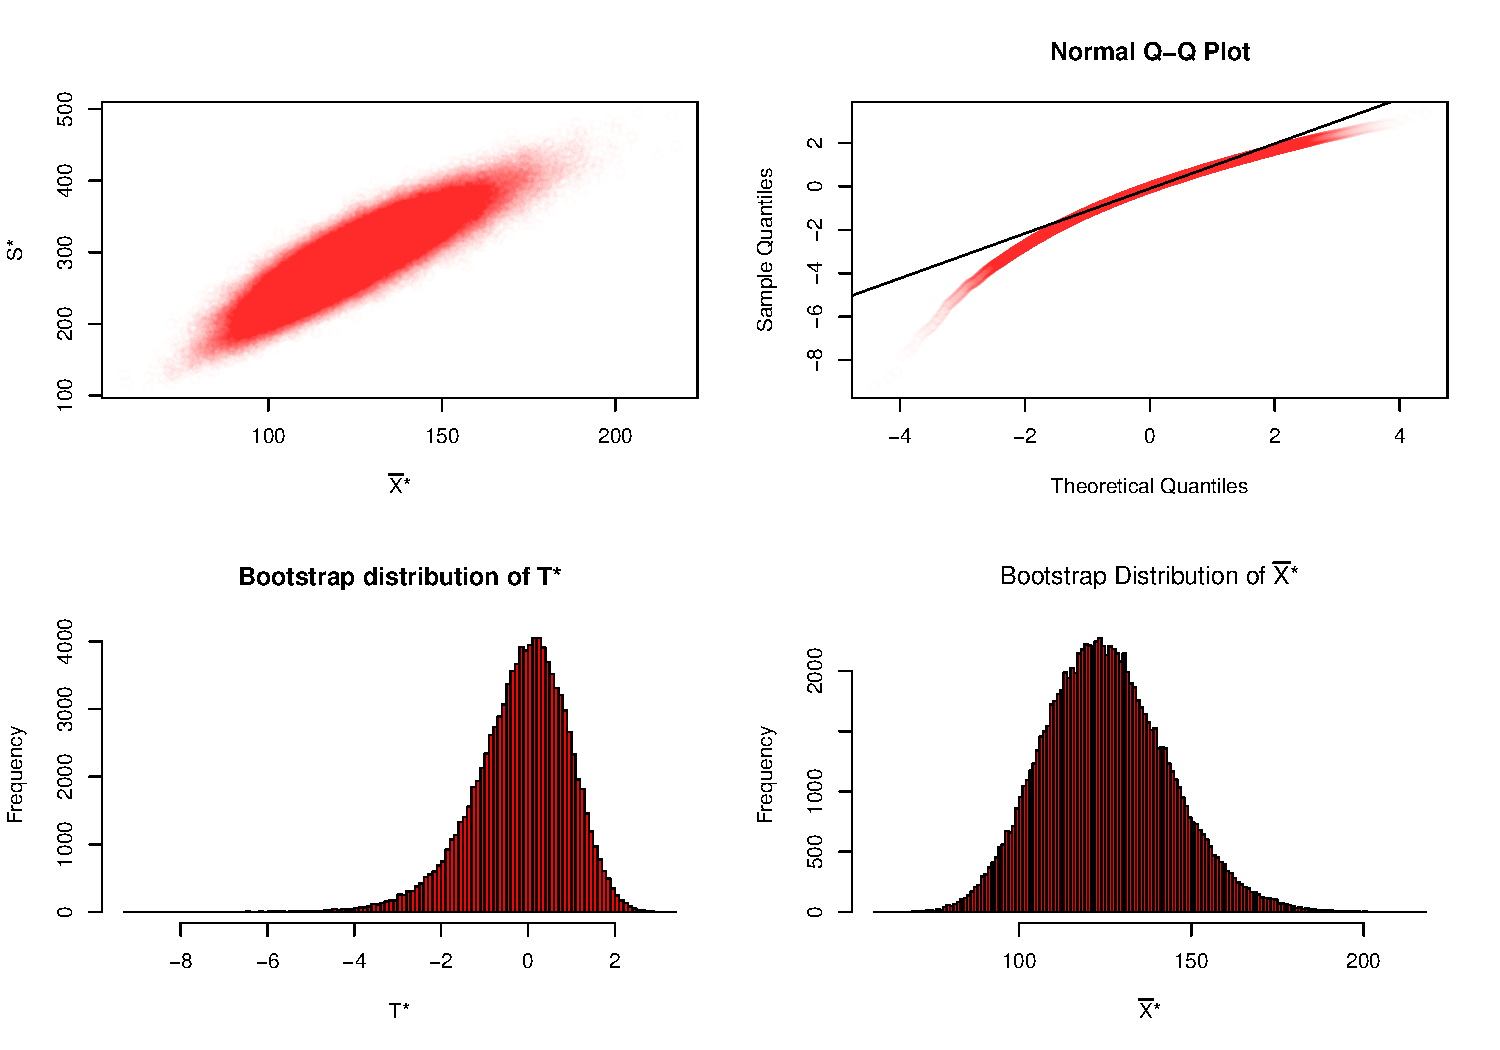
\includegraphics[width=0.9\linewidth,height=0.9\textheight]{Week5_Lect_files/figure-beamer/unnamed-chunk-26-1} \end{center}
\end{frame}

\begin{frame}[fragile]{Observed/fitted values and residuals}
\protect\hypertarget{observedfitted-values-and-residuals-1}{}
\begin{itemize}
\item
  We'll compute the observed values, fitted values, and residuals for
  the interaction model which we saved in
  \texttt{score\_model\_interaction}.

  \begin{itemize}
  \tightlist
  \item
    Say, you have an instructor who identifies as female and is 36 years
    old. What fitted value \(\hat{y}=\widehat{\text{score}}\) would our
    model yield?
  \item
    Say, you have another instructor who identifies as male and is 59
    years old. What would their fitted value \(\hat{y}\) be?
  \end{itemize}
\item
  See if you can answer this question visually.
\end{itemize}

\begin{center}\includegraphics[width=0.8\linewidth,height=0.45\textheight]{Week5_Lect_files/figure-beamer/unnamed-chunk-27-1} \end{center}
\end{frame}

\begin{frame}{Observed/fitted values and residuals}
\protect\hypertarget{observedfitted-values-and-residuals-2}{}
\begin{itemize}
\tightlist
\item
  For female instructors, we have.
\end{itemize}

\[\begin{array}{ll}
\hat{y}=\widehat{\text{score}}&=4.883-0.018\cdot \text{age}\\
&=4.883-0.018\cdot 36=4.24
\end{array}\]

\begin{itemize}
\tightlist
\item
  For male instructors.
\end{itemize}

\[\begin{array}{ll}
\hat{y}=\widehat{\text{score}}&=4.437-0.004\cdot \text{age}\\
&=4.437-0.004\cdot 59=4.20
\end{array}\]
\end{frame}

\begin{frame}[fragile]{Observed/fitted values and residuals}
\protect\hypertarget{observedfitted-values-and-residuals-3}{}
Note: It is better to let R compute the values and round at the end.

\normalsize

\begin{Shaded}
\begin{Highlighting}[]
\FunctionTok{predict}\NormalTok{(score\_model\_interaction, }
        \AttributeTok{newdata =} \FunctionTok{data.frame}\NormalTok{(}\AttributeTok{age =} \DecValTok{36}\NormalTok{, }\AttributeTok{gender =} \StringTok{"female"}\NormalTok{))}
\end{Highlighting}
\end{Shaded}

\begin{verbatim}
       1 
4.252148 
\end{verbatim}

\begin{Shaded}
\begin{Highlighting}[]
\FunctionTok{predict}\NormalTok{(score\_model\_interaction, }
        \AttributeTok{newdata =} \FunctionTok{data.frame}\NormalTok{(}\AttributeTok{age =} \DecValTok{59}\NormalTok{, }\AttributeTok{gender =} \StringTok{"male"}\NormalTok{))}
\end{Highlighting}
\end{Shaded}

\begin{verbatim}
       1 
4.201373 
\end{verbatim}

\normalsize
\end{frame}

\begin{frame}{Example: One numerical and one categorical explanatory
variable}
\protect\hypertarget{example-one-numerical-and-one-categorical-explanatory-variable}{}
\begin{tcolorbox}
Suppose a realtor wants to model the appraised price of an apartment as a function of the predictors living area (in $\text{m}^2$) and the presence or absence of elevators. Consider the data frame `VIT2005`, which contains data about apartments in Vitoria, Spain, including \textbf{totalprice}, \textbf{area}, and \textbf{elevator}, which are the appraised apartment value in Euros, living space in square meters, and the absence or presence of at least one elevator in the building, respectively. The realtor first wants to know if there is any relationship between appraised price ($Y$) and living area ($x_1$). Next, the realtor wants to know how adding a dummy variable for whether or not an elevator is present changes the relationship: Are the lines the same? Are the slopes the same? Are the intercepts the same?
\end{tcolorbox}
\end{frame}

\begin{frame}[fragile]{Solution (is there a realationship between
\texttt{totalprice} and \texttt{area}?):}
\protect\hypertarget{solution-is-there-a-realationship-between-totalprice-and-area}{}
\normalsize

\begin{Shaded}
\begin{Highlighting}[]
\FunctionTok{library}\NormalTok{(PASWR2)}
\NormalTok{VIT2005 }\OtherTok{\textless{}{-}}\NormalTok{ VIT2005 }\SpecialCharTok{\%\textgreater{}\%} 
  \FunctionTok{mutate}\NormalTok{(}\AttributeTok{elevator =} \FunctionTok{factor}\NormalTok{(elevator, }\AttributeTok{labels =} \FunctionTok{c}\NormalTok{(}\StringTok{"No"}\NormalTok{, }\StringTok{"Yes"}\NormalTok{)))}
\FunctionTok{ggplot}\NormalTok{(}\AttributeTok{data =}\NormalTok{ VIT2005, }\FunctionTok{aes}\NormalTok{(}\AttributeTok{x =}\NormalTok{ area, }\AttributeTok{y =}\NormalTok{ totalprice)) }\SpecialCharTok{+} 
  \FunctionTok{geom\_point}\NormalTok{() }\SpecialCharTok{+} 
  \FunctionTok{theme\_bw}\NormalTok{() }\SpecialCharTok{+}
  \FunctionTok{geom\_smooth}\NormalTok{(}\AttributeTok{method =} \StringTok{"lm"}\NormalTok{, }\AttributeTok{se =} \ConstantTok{FALSE}\NormalTok{)}
\end{Highlighting}
\end{Shaded}

\begin{center}\includegraphics[width=0.7\linewidth,height=0.4\textheight]{Week5_Lect_files/figure-beamer/unnamed-chunk-29-1} \end{center}
\normalsize
\end{frame}

\begin{frame}[fragile]{Solution (is there a realationship between
\texttt{totalprice} and \texttt{area}?):}
\protect\hypertarget{solution-is-there-a-realationship-between-totalprice-and-area-1}{}
\scriptsize

\begin{Shaded}
\begin{Highlighting}[]
\NormalTok{mod\_simple }\OtherTok{\textless{}{-}} \FunctionTok{lm}\NormalTok{(totalprice }\SpecialCharTok{\textasciitilde{}}\NormalTok{ area, }\AttributeTok{data =}\NormalTok{ VIT2005)}
\FunctionTok{summary}\NormalTok{(mod\_simple)}
\end{Highlighting}
\end{Shaded}

\begin{verbatim}

Call:
lm(formula = totalprice ~ area, data = VIT2005)

Residuals:
    Min      1Q  Median      3Q     Max 
-156126  -21564   -2155   19493  120674 

Coefficients:
            Estimate Std. Error t value Pr(>|t|)    
(Intercept)  40822.4    12170.1   3.354  0.00094 ***
area          2704.8      133.6  20.243  < 2e-16 ***
---
Signif. codes:  0 '***' 0.001 '**' 0.01 '*' 0.05 '.' 0.1 ' ' 1

Residual standard error: 40810 on 216 degrees of freedom
Multiple R-squared:  0.6548,    Adjusted R-squared:  0.6532 
F-statistic: 409.8 on 1 and 216 DF,  p-value: < 2.2e-16
\end{verbatim}

\normalsize
\end{frame}

\begin{frame}[fragile]{Solution (is there a realationship between
\texttt{totalprice} and \texttt{area}?):}
\protect\hypertarget{solution-is-there-a-realationship-between-totalprice-and-area-2}{}
\normalsize

\begin{Shaded}
\begin{Highlighting}[]
\NormalTok{knitr}\SpecialCharTok{::}\FunctionTok{kable}\NormalTok{(}\FunctionTok{get\_regression\_table}\NormalTok{(mod\_simple))}
\end{Highlighting}
\end{Shaded}

\begin{longtable}[]{@{}
  >{\raggedright\arraybackslash}p{(\columnwidth - 12\tabcolsep) * \real{0.1471}}
  >{\raggedleft\arraybackslash}p{(\columnwidth - 12\tabcolsep) * \real{0.1471}}
  >{\raggedleft\arraybackslash}p{(\columnwidth - 12\tabcolsep) * \real{0.1471}}
  >{\raggedleft\arraybackslash}p{(\columnwidth - 12\tabcolsep) * \real{0.1471}}
  >{\raggedleft\arraybackslash}p{(\columnwidth - 12\tabcolsep) * \real{0.1176}}
  >{\raggedleft\arraybackslash}p{(\columnwidth - 12\tabcolsep) * \real{0.1471}}
  >{\raggedleft\arraybackslash}p{(\columnwidth - 12\tabcolsep) * \real{0.1471}}@{}}
\toprule\noalign{}
\begin{minipage}[b]{\linewidth}\raggedright
term
\end{minipage} & \begin{minipage}[b]{\linewidth}\raggedleft
estimate
\end{minipage} & \begin{minipage}[b]{\linewidth}\raggedleft
std\_error
\end{minipage} & \begin{minipage}[b]{\linewidth}\raggedleft
statistic
\end{minipage} & \begin{minipage}[b]{\linewidth}\raggedleft
p\_value
\end{minipage} & \begin{minipage}[b]{\linewidth}\raggedleft
lower\_ci
\end{minipage} & \begin{minipage}[b]{\linewidth}\raggedleft
upper\_ci
\end{minipage} \\
\midrule\noalign{}
\endhead
intercept & 40822.416 & 12170.092 & 3.354 & 0.001 & 16835.075 &
64809.757 \\
area & 2704.751 & 133.616 & 20.243 & 0.000 & 2441.393 & 2968.109 \\
\bottomrule\noalign{}
\end{longtable}

\normalsize
\end{frame}

\begin{frame}[fragile]{Solution (does adding a dummy variable
(\texttt{elevator}) change the relationship?):}
\protect\hypertarget{solution-does-adding-a-dummy-variable-elevator-change-the-relationship}{}
\scriptsize

\begin{Shaded}
\begin{Highlighting}[]
\FunctionTok{ggplot}\NormalTok{(VIT2005, }\FunctionTok{aes}\NormalTok{(}\AttributeTok{x =}\NormalTok{ area, }\AttributeTok{y =}\NormalTok{ totalprice, }\AttributeTok{color =}\NormalTok{ elevator)) }\SpecialCharTok{+}
  \FunctionTok{geom\_point}\NormalTok{() }\SpecialCharTok{+}
  \FunctionTok{labs}\NormalTok{(}\AttributeTok{x =} \StringTok{"Area (sq meters)"}\NormalTok{, }\AttributeTok{y =} \StringTok{"Total Price (euros)"}\NormalTok{, }
       \AttributeTok{color =} \StringTok{"Elevator"}\NormalTok{) }\SpecialCharTok{+}
  \FunctionTok{geom\_smooth}\NormalTok{(}\AttributeTok{method =} \StringTok{"lm"}\NormalTok{, }\AttributeTok{se =} \ConstantTok{FALSE}\NormalTok{) }\SpecialCharTok{+} 
  \FunctionTok{theme\_bw}\NormalTok{()}
\end{Highlighting}
\end{Shaded}

\begin{center}\includegraphics[width=0.8\linewidth,height=0.5\textheight]{Week5_Lect_files/figure-beamer/unnamed-chunk-32-1} \end{center}
\normalsize
\end{frame}

\begin{frame}[fragile]{Solution (does adding a dummy variable
(\texttt{elevator}) change the relationship?):}
\protect\hypertarget{solution-does-adding-a-dummy-variable-elevator-change-the-relationship-1}{}
\scriptsize

\begin{Shaded}
\begin{Highlighting}[]
\NormalTok{mod\_int }\OtherTok{\textless{}{-}} \FunctionTok{lm}\NormalTok{(totalprice }\SpecialCharTok{\textasciitilde{}}\NormalTok{ area }\SpecialCharTok{+}\NormalTok{ elevator }\SpecialCharTok{+}\NormalTok{ area}\SpecialCharTok{:}\NormalTok{elevator, }\AttributeTok{data =}\NormalTok{ VIT2005)}
\FunctionTok{summary}\NormalTok{(mod\_int)}
\end{Highlighting}
\end{Shaded}

\begin{verbatim}

Call:
lm(formula = totalprice ~ area + elevator + area:elevator, data = VIT2005)

Residuals:
    Min      1Q  Median      3Q     Max 
-133610  -22216   -2423   20276  113159 

Coefficients:
                 Estimate Std. Error t value Pr(>|t|)    
(Intercept)      113114.0    28985.0   3.902 0.000128 ***
area               1343.7      392.2   3.426 0.000735 ***
elevatorYes      -50871.7    31990.6  -1.590 0.113264    
area:elevatorYes   1202.0      417.4   2.880 0.004380 ** 
---
Signif. codes:  0 '***' 0.001 '**' 0.01 '*' 0.05 '.' 0.1 ' ' 1

Residual standard error: 37610 on 214 degrees of freedom
Multiple R-squared:  0.7096,    Adjusted R-squared:  0.7055 
F-statistic: 174.3 on 3 and 214 DF,  p-value: < 2.2e-16
\end{verbatim}

\normalsize
\end{frame}

\begin{frame}[fragile]{Solution (does adding a dummy variable
(\texttt{elevator}) change the relationship?):}
\protect\hypertarget{solution-does-adding-a-dummy-variable-elevator-change-the-relationship-2}{}
\scriptsize

\begin{Shaded}
\begin{Highlighting}[]
\NormalTok{mod\_ps }\OtherTok{\textless{}{-}} \FunctionTok{lm}\NormalTok{(totalprice }\SpecialCharTok{\textasciitilde{}}\NormalTok{ area }\SpecialCharTok{+}\NormalTok{ elevator, }\AttributeTok{data =}\NormalTok{ VIT2005)}
\FunctionTok{summary}\NormalTok{(mod\_ps)}
\end{Highlighting}
\end{Shaded}

\begin{verbatim}

Call:
lm(formula = totalprice ~ area + elevator, data = VIT2005)

Residuals:
    Min      1Q  Median      3Q     Max 
-120265  -20224   -2567   18281  112406 

Coefficients:
            Estimate Std. Error t value Pr(>|t|)    
(Intercept)  36173.6    11434.8   3.163  0.00178 ** 
area          2405.4      136.3  17.652  < 2e-16 ***
elevatorYes  39091.1     7022.8   5.566 7.71e-08 ***
---
Signif. codes:  0 '***' 0.001 '**' 0.01 '*' 0.05 '.' 0.1 ' ' 1

Residual standard error: 38240 on 215 degrees of freedom
Multiple R-squared:  0.6983,    Adjusted R-squared:  0.6955 
F-statistic: 248.8 on 2 and 215 DF,  p-value: < 2.2e-16
\end{verbatim}

\normalsize
\end{frame}

\begin{frame}[fragile]{Diagnostic Plots}
\protect\hypertarget{diagnostic-plots}{}
\small

\begin{Shaded}
\begin{Highlighting}[]
\FunctionTok{library}\NormalTok{(ggfortify)}
\FunctionTok{autoplot}\NormalTok{(mod\_int, }\AttributeTok{ncol =} \DecValTok{2}\NormalTok{, }\AttributeTok{nrow =} \DecValTok{1}\NormalTok{, }\AttributeTok{which =} \DecValTok{1}\SpecialCharTok{:}\DecValTok{2}\NormalTok{) }\SpecialCharTok{+} 
  \FunctionTok{theme\_bw}\NormalTok{()}
\end{Highlighting}
\end{Shaded}

\begin{center}\includegraphics[width=0.8\linewidth,height=0.5\textheight]{Week5_Lect_files/figure-beamer/unnamed-chunk-35-1} \end{center}
\normalsize
\end{frame}

\hypertarget{two-numerical-explanatory-variables}{%
\section{Two numerical explanatory
variables}\label{two-numerical-explanatory-variables}}

\begin{frame}[fragile]{Two numerical explanatory variables}
\protect\hypertarget{two-numerical-explanatory-variables-1}{}
\begin{itemize}
\item
  Let's switch gears and consider multiple regression models where
  instead of one numerical and one categorical explanatory variable, we
  have two numerical explanatory variables.
\item
  The \texttt{Credit} dataset we will use is from the \texttt{ISLR}
  package.

  \begin{itemize}
  \tightlist
  \item
    The outcome variable of interest is the credit card debt of 400
    individuals.
  \item
    Other variables like income, credit limit, credit rating, and age
    are included as well.
  \end{itemize}
\item
  Note that the \texttt{Credit} data is not based on real individuals'
  financial information, but rather is a simulated dataset used for
  educational purposes.
\end{itemize}
\end{frame}

\begin{frame}[fragile]{Exploratory data analysis}
\protect\hypertarget{exploratory-data-analysis-14}{}
Use \texttt{select()} to create a subset of the variables we'll consider
in this chapter.

\small

\begin{Shaded}
\begin{Highlighting}[]
\FunctionTok{library}\NormalTok{(ISLR)}
\NormalTok{credit\_ch6 }\OtherTok{\textless{}{-}}\NormalTok{ Credit }\SpecialCharTok{\%\textgreater{}\%} 
  \FunctionTok{as\_tibble}\NormalTok{() }\SpecialCharTok{\%\textgreater{}\%} 
  \FunctionTok{select}\NormalTok{(ID, }\AttributeTok{debt =}\NormalTok{ Balance, }\AttributeTok{credit\_limit =}\NormalTok{ Limit, }
         \AttributeTok{income =}\NormalTok{ Income, }\AttributeTok{credit\_rating =}\NormalTok{ Rating, }\AttributeTok{age =}\NormalTok{ Age)}
\FunctionTok{glimpse}\NormalTok{(credit\_ch6)}
\end{Highlighting}
\end{Shaded}

\begin{verbatim}
Rows: 400
Columns: 6
$ ID            <int> 1, 2, 3, 4, 5, 6, 7, 8, 9, 10, 11, 12, 13, 14, 15, 16, 1~
$ debt          <int> 333, 903, 580, 964, 331, 1151, 203, 872, 279, 1350, 1407~
$ credit_limit  <int> 3606, 6645, 7075, 9504, 4897, 8047, 3388, 7114, 3300, 68~
$ income        <dbl> 14.891, 106.025, 104.593, 148.924, 55.882, 80.180, 20.99~
$ credit_rating <int> 283, 483, 514, 681, 357, 569, 259, 512, 266, 491, 589, 1~
$ age           <int> 34, 82, 71, 36, 68, 77, 37, 87, 66, 41, 30, 64, 57, 49, ~
\end{verbatim}

\normalsize
\end{frame}

\begin{frame}[fragile]{Exploratory data analysis}
\protect\hypertarget{exploratory-data-analysis-15}{}
\normalsize

\begin{Shaded}
\begin{Highlighting}[]
\NormalTok{credit\_ch6 }\SpecialCharTok{\%\textgreater{}\%} 
  \FunctionTok{sample\_n}\NormalTok{(}\AttributeTok{size =} \DecValTok{5}\NormalTok{)}
\end{Highlighting}
\end{Shaded}

\begin{verbatim}
# A tibble: 5 x 6
     ID  debt credit_limit income credit_rating   age
  <int> <int>        <int>  <dbl>         <int> <int>
1   101   298         3736   21.2           256    41
2   236   191         2923   10.5           232    25
3    83   503         4433   23.7           344    63
4   357   962         6090   34.5           442    36
5   115   271         3326   16.5           268    41
\end{verbatim}

\normalsize

\normalsize

\begin{Shaded}
\begin{Highlighting}[]
\NormalTok{credit\_ch6 }\SpecialCharTok{\%\textgreater{}\%} 
  \FunctionTok{select}\NormalTok{(debt, credit\_limit, income) }\SpecialCharTok{\%\textgreater{}\%} 
  \FunctionTok{skim}\NormalTok{()}
\end{Highlighting}
\end{Shaded}
\end{frame}

\begin{frame}[fragile]{Exploratory data analysis}
\protect\hypertarget{exploratory-data-analysis-16}{}
\normalsize

\begin{Shaded}
\begin{Highlighting}[]
\NormalTok{credit\_ch6 }\SpecialCharTok{\%\textgreater{}\%} 
  \FunctionTok{select}\NormalTok{(debt, credit\_limit, income) }\SpecialCharTok{\%\textgreater{}\%} 
  \FunctionTok{summary}\NormalTok{()}
\end{Highlighting}
\end{Shaded}

\begin{verbatim}
      debt          credit_limit       income      
 Min.   :   0.00   Min.   :  855   Min.   : 10.35  
 1st Qu.:  68.75   1st Qu.: 3088   1st Qu.: 21.01  
 Median : 459.50   Median : 4622   Median : 33.12  
 Mean   : 520.01   Mean   : 4736   Mean   : 45.22  
 3rd Qu.: 863.00   3rd Qu.: 5873   3rd Qu.: 57.47  
 Max.   :1999.00   Max.   :13913   Max.   :186.63  
\end{verbatim}

\normalsize
\end{frame}

\begin{frame}[fragile]{Exploratory data analysis}
\protect\hypertarget{exploratory-data-analysis-17}{}
We can compute the correlation coefficient between the different
possible pairs of these variables.

\normalsize

\begin{Shaded}
\begin{Highlighting}[]
\NormalTok{credit\_ch6 }\SpecialCharTok{\%\textgreater{}\%} 
  \FunctionTok{select}\NormalTok{(debt, credit\_limit, income) }\SpecialCharTok{\%\textgreater{}\%} 
  \FunctionTok{cor}\NormalTok{()}
\end{Highlighting}
\end{Shaded}

\begin{verbatim}
                  debt credit_limit    income
debt         1.0000000    0.8616973 0.4636565
credit_limit 0.8616973    1.0000000 0.7920883
income       0.4636565    0.7920883 1.0000000
\end{verbatim}

\normalsize
\end{frame}

\begin{frame}[fragile]{Exploratory data analysis}
\protect\hypertarget{exploratory-data-analysis-18}{}
\small

\begin{Shaded}
\begin{Highlighting}[]
\FunctionTok{library}\NormalTok{(psych)}
\FunctionTok{pairs.panels}\NormalTok{(credit\_ch6[, }\DecValTok{2}\SpecialCharTok{:}\DecValTok{4}\NormalTok{],  }\CommentTok{\# select debt (2), credit\_limit (3), }
             \CommentTok{\# income (4)}
             \AttributeTok{method =} \StringTok{"pearson"}\NormalTok{, }\CommentTok{\# correlation method}
             \AttributeTok{hist.col =} \StringTok{"lightblue"}\NormalTok{,}
             \AttributeTok{density =} \ConstantTok{TRUE}\NormalTok{,  }\CommentTok{\# show density plots}
             \AttributeTok{ellipses =} \ConstantTok{FALSE} \CommentTok{\# show correlation ellipses}
\NormalTok{             )}
\end{Highlighting}
\end{Shaded}

\begin{center}\includegraphics[width=0.6\linewidth,height=0.45\textheight]{Week5_Lect_files/figure-beamer/unnamed-chunk-41-1} \end{center}
\normalsize
\end{frame}

\begin{frame}[fragile]{Exploratory data analysis: Collinearity}
\protect\hypertarget{exploratory-data-analysis-collinearity}{}
\begin{itemize}
\item
  We say there is a high degree of collinearity between the
  \texttt{credit\_limit} and \texttt{income} explanatory variables.
\item
  Collinearity (or multicollinearity) is a phenomenon where one
  explanatory variable in a multiple regression model is \textbf{highly
  correlated with another}.
\item
  So in our case since \texttt{credit\_limit} and \texttt{income} are
  highly correlated.

  \begin{itemize}
  \tightlist
  \item
    If we knew a persons' \texttt{credit\_limit}, we could make a pretty
    good guess about their \texttt{income}.
  \item
    Thus, these two variables provide somewhat redundant information.
  \end{itemize}
\item
  We will leave discussion on how to work with collinear explanatory
  variables for another course.
\end{itemize}
\end{frame}

\begin{frame}[fragile]{Exploratory data analysis: visualization}
\protect\hypertarget{exploratory-data-analysis-visualization}{}
Let's visualize the relationship of the outcome variable with each of
the two explanatory variables in two separate plots

\normalsize

\begin{Shaded}
\begin{Highlighting}[]
\FunctionTok{ggplot}\NormalTok{(}\AttributeTok{data =}\NormalTok{ credit\_ch6, }\FunctionTok{aes}\NormalTok{(}\AttributeTok{x =}\NormalTok{ credit\_limit, }\AttributeTok{y =}\NormalTok{ debt)) }\SpecialCharTok{+} 
  \FunctionTok{geom\_point}\NormalTok{() }\SpecialCharTok{+} 
  \FunctionTok{labs}\NormalTok{(}\AttributeTok{x=} \StringTok{"Credit limit (in$)"}\NormalTok{, }\AttributeTok{y =} \StringTok{"Credit card debt (in$)"}\NormalTok{, }
       \AttributeTok{title =} \StringTok{"Debt and Credit Limit"}\NormalTok{) }\SpecialCharTok{+} 
  \FunctionTok{geom\_smooth}\NormalTok{(}\AttributeTok{method =} \StringTok{"lm"}\NormalTok{, }\AttributeTok{se =} \ConstantTok{FALSE}\NormalTok{) }\SpecialCharTok{+} 
  \FunctionTok{theme\_bw}\NormalTok{() }\OtherTok{{-}\textgreater{}}\NormalTok{ p1}
\FunctionTok{ggplot}\NormalTok{(}\AttributeTok{data =}\NormalTok{ credit\_ch6, }\FunctionTok{aes}\NormalTok{(}\AttributeTok{x =}\NormalTok{ income, }\AttributeTok{y =}\NormalTok{ debt)) }\SpecialCharTok{+} 
  \FunctionTok{geom\_point}\NormalTok{() }\SpecialCharTok{+} 
  \FunctionTok{labs}\NormalTok{(}\AttributeTok{x =} \StringTok{"Income (in $1000)"}\NormalTok{, }\AttributeTok{y =} \StringTok{"Credit card debt (in $)"}\NormalTok{,}
       \AttributeTok{title =} \StringTok{"Debt and Income"}\NormalTok{) }\SpecialCharTok{+}
  \FunctionTok{geom\_smooth}\NormalTok{(}\AttributeTok{method =} \StringTok{"lm"}\NormalTok{, }\AttributeTok{se =} \ConstantTok{FALSE}\NormalTok{) }\SpecialCharTok{+} 
  \FunctionTok{theme\_bw}\NormalTok{() }\OtherTok{{-}\textgreater{}}\NormalTok{ p2}
\FunctionTok{library}\NormalTok{(patchwork)}
\NormalTok{p1 }\SpecialCharTok{+}\NormalTok{ p2}
\end{Highlighting}
\end{Shaded}

\normalsize
\end{frame}

\begin{frame}{Exploratory data analysis: visualization}
\protect\hypertarget{exploratory-data-analysis-visualization-1}{}
\begin{center}\includegraphics[width=0.9\linewidth,height=0.9\textheight]{Week5_Lect_files/figure-beamer/unnamed-chunk-43-1} \end{center}
\end{frame}

\begin{frame}[fragile]{Exploratory data analysis: visualization}
\protect\hypertarget{exploratory-data-analysis-visualization-2}{}
To visualize the joint relationship of all three variables
simultaneously, we need a 3-dimensional (3D) scatterplot. The following
code will create a 3-dimensional scatterplot.

\begin{Shaded}
\begin{Highlighting}[]
\FunctionTok{library}\NormalTok{(plotly)}
\NormalTok{p }\OtherTok{\textless{}{-}} \FunctionTok{plot\_ly}\NormalTok{(}\AttributeTok{data =}\NormalTok{ credit\_ch6, }\AttributeTok{z =} \SpecialCharTok{\textasciitilde{}}\NormalTok{debt, }\AttributeTok{x =} \SpecialCharTok{\textasciitilde{}}\NormalTok{credit\_limit, }
             \AttributeTok{y =} \SpecialCharTok{\textasciitilde{}}\NormalTok{income) }\SpecialCharTok{\%\textgreater{}\%} \FunctionTok{add\_markers}\NormalTok{()}
\NormalTok{mod }\OtherTok{\textless{}{-}} \FunctionTok{lm}\NormalTok{(debt }\SpecialCharTok{\textasciitilde{}}\NormalTok{ credit\_limit }\SpecialCharTok{+}\NormalTok{ income, }\AttributeTok{data =}\NormalTok{ credit\_ch6)}
\NormalTok{x }\OtherTok{\textless{}{-}} \FunctionTok{seq}\NormalTok{(}\FunctionTok{min}\NormalTok{(credit\_ch6}\SpecialCharTok{$}\NormalTok{credit\_limit), }
         \FunctionTok{max}\NormalTok{(credit\_ch6}\SpecialCharTok{$}\NormalTok{credit\_limit), }\AttributeTok{length =} \DecValTok{70}\NormalTok{)}
\NormalTok{y }\OtherTok{\textless{}{-}} \FunctionTok{seq}\NormalTok{(}\FunctionTok{min}\NormalTok{(credit\_ch6}\SpecialCharTok{$}\NormalTok{income), }
         \FunctionTok{max}\NormalTok{(credit\_ch6}\SpecialCharTok{$}\NormalTok{income), }\AttributeTok{length =} \DecValTok{70}\NormalTok{) }
\NormalTok{plane }\OtherTok{\textless{}{-}} \FunctionTok{outer}\NormalTok{(x, y, }\ControlFlowTok{function}\NormalTok{(a, b)\{}\FunctionTok{coef}\NormalTok{(mod)[}\DecValTok{1}\NormalTok{] }\SpecialCharTok{+} 
               \FunctionTok{coef}\NormalTok{(mod)[}\DecValTok{2}\NormalTok{]}\SpecialCharTok{*}\NormalTok{a }\SpecialCharTok{+} \FunctionTok{coef}\NormalTok{(mod)[}\DecValTok{3}\NormalTok{]}\SpecialCharTok{*}\NormalTok{b\})}
\CommentTok{\# draw the plane}
\NormalTok{p }\SpecialCharTok{\%\textgreater{}\%} 
  \FunctionTok{add\_surface}\NormalTok{(}\AttributeTok{x =} \SpecialCharTok{\textasciitilde{}}\NormalTok{x, }\AttributeTok{y =} \SpecialCharTok{\textasciitilde{}}\NormalTok{y, }\AttributeTok{z =} \SpecialCharTok{\textasciitilde{}}\NormalTok{plane)}
\end{Highlighting}
\end{Shaded}
\end{frame}

\begin{frame}{Exploratory data analysis: visualization}
\protect\hypertarget{exploratory-data-analysis-visualization-3}{}
\begin{center}\includegraphics[width=0.7\linewidth,height=0.5\textheight]{week5_7} \end{center}

The regression plane is the ``best-fitting'' plane that similarly
minimizes the sum of squared residuals.
\end{frame}

\begin{frame}[fragile]{Regression plane}
\protect\hypertarget{regression-plane}{}
\footnotesize

\begin{Shaded}
\begin{Highlighting}[]
\CommentTok{\# Fit regression model:}
\NormalTok{debt\_model }\OtherTok{\textless{}{-}} \FunctionTok{lm}\NormalTok{(debt }\SpecialCharTok{\textasciitilde{}}\NormalTok{ credit\_limit }\SpecialCharTok{+}\NormalTok{ income, }
                 \AttributeTok{data =}\NormalTok{ credit\_ch6)}
\CommentTok{\# Get regression table:}
\NormalTok{knitr}\SpecialCharTok{::}\FunctionTok{kable}\NormalTok{(}\FunctionTok{get\_regression\_table}\NormalTok{(debt\_model))     }
\end{Highlighting}
\end{Shaded}

\begin{longtable}[]{@{}
  >{\raggedright\arraybackslash}p{(\columnwidth - 12\tabcolsep) * \real{0.1912}}
  >{\raggedleft\arraybackslash}p{(\columnwidth - 12\tabcolsep) * \real{0.1324}}
  >{\raggedleft\arraybackslash}p{(\columnwidth - 12\tabcolsep) * \real{0.1471}}
  >{\raggedleft\arraybackslash}p{(\columnwidth - 12\tabcolsep) * \real{0.1471}}
  >{\raggedleft\arraybackslash}p{(\columnwidth - 12\tabcolsep) * \real{0.1176}}
  >{\raggedleft\arraybackslash}p{(\columnwidth - 12\tabcolsep) * \real{0.1324}}
  >{\raggedleft\arraybackslash}p{(\columnwidth - 12\tabcolsep) * \real{0.1324}}@{}}
\toprule\noalign{}
\begin{minipage}[b]{\linewidth}\raggedright
term
\end{minipage} & \begin{minipage}[b]{\linewidth}\raggedleft
estimate
\end{minipage} & \begin{minipage}[b]{\linewidth}\raggedleft
std\_error
\end{minipage} & \begin{minipage}[b]{\linewidth}\raggedleft
statistic
\end{minipage} & \begin{minipage}[b]{\linewidth}\raggedleft
p\_value
\end{minipage} & \begin{minipage}[b]{\linewidth}\raggedleft
lower\_ci
\end{minipage} & \begin{minipage}[b]{\linewidth}\raggedleft
upper\_ci
\end{minipage} \\
\midrule\noalign{}
\endhead
intercept & -385.179 & 19.465 & -19.789 & 0 & -423.446 & -346.912 \\
credit\_limit & 0.264 & 0.006 & 44.955 & 0 & 0.253 & 0.276 \\
income & -7.663 & 0.385 & -19.901 & 0 & -8.420 & -6.906 \\
\bottomrule\noalign{}
\end{longtable}

\normalsize
\end{frame}

\begin{frame}[fragile]{Regression plane: Interpretation}
\protect\hypertarget{regression-plane-interpretation}{}
\begin{itemize}
\item
  First, the intercept value is \(-\$385.179\).

  \begin{itemize}
  \tightlist
  \item
    This intercept represents the credit card debt for an individual who
    has \texttt{credit\_limit} of \(\$0\) and income of \(\$0\).
  \item
    In our data, the intercept has no practical interpretation since no
    individuals had both \texttt{credit\_limit} an \texttt{income}
    values of \(\$0\).
  \item
    Rather, the intercept is used to situate the regression plane in 3D
    space.
  \end{itemize}
\item
  Second, the \texttt{credit\_limit} value is \(\$0.264\).

  \begin{itemize}
  \tightlist
  \item
    Taking into account all the other explanatory variables in our
    model, for every increase of one dollar in \texttt{credit\_limit},
    there is an associated increase of on average \(\$0.26\) in credit
    card debt.
  \item
    Just as we earlier, we are cautious not to imply causality. We do
    this merely stating there was an associated increase.
  \end{itemize}
\item
  Third, income = \(-\$7.66\).

  \begin{itemize}
  \tightlist
  \item
    Taking into account all other explanatory variables in our model,
    for every increase of one unit of income (\(\$1000\) in actual
    income), there is an associated decrease of, on average, \(\$7.66\)
    in credit card debt.
  \end{itemize}
\end{itemize}
\end{frame}

\begin{frame}{Regression plane: Prediction}
\protect\hypertarget{regression-plane-prediction}{}
Putting these results together, the equation of the regression plane
that gives us fitted values \(\hat{y}=\widehat{\text{debt}}\) is:

\[\begin{array}{ll}
\hat{y}&=b_0+b_1\cdot x_1+b_2\cdot x_2\\
\widehat{\text{debt}}&=b_0+b_{limit}\cdot \text{limit}+b_{income}\cdot \text{income}\\
&=-385.179+0.263 \cdot \text{limit}- 7.663\cdot \text{income}
\end{array}\]
\end{frame}

\begin{frame}[fragile]{Diagnostic Plots}
\protect\hypertarget{diagnostic-plots-1}{}
\normalsize

\begin{Shaded}
\begin{Highlighting}[]
\FunctionTok{autoplot}\NormalTok{(debt\_model, }\AttributeTok{ncol =} \DecValTok{2}\NormalTok{, }\AttributeTok{nrow =} \DecValTok{1}\NormalTok{, }\AttributeTok{which =} \DecValTok{1}\SpecialCharTok{:}\DecValTok{2}\NormalTok{) }\SpecialCharTok{+} 
  \FunctionTok{theme\_bw}\NormalTok{()}
\end{Highlighting}
\end{Shaded}

\begin{center}\includegraphics[width=0.8\linewidth,height=0.5\textheight]{Week5_Lect_files/figure-beamer/unnamed-chunk-47-1} \end{center}
\normalsize
\end{frame}

\begin{frame}[fragile]{Simpson's Paradox}
\protect\hypertarget{simpsons-paradox}{}
\tiny

\begin{Shaded}
\begin{Highlighting}[]
\FunctionTok{library}\NormalTok{(ISLR)}
\NormalTok{credit\_paradox }\OtherTok{\textless{}{-}}\NormalTok{ Credit }\SpecialCharTok{\%\textgreater{}\%} 
  \FunctionTok{select}\NormalTok{(ID, }\AttributeTok{debt =}\NormalTok{ Balance, }\AttributeTok{credit\_limit =}\NormalTok{ Limit, }
         \AttributeTok{credit\_rating =}\NormalTok{ Rating, }\AttributeTok{income =}\NormalTok{ Income, }\AttributeTok{age =}\NormalTok{ Age)}
\FunctionTok{ggplot}\NormalTok{(}\AttributeTok{data =}\NormalTok{ credit\_paradox, }\FunctionTok{aes}\NormalTok{(}\AttributeTok{x =}\NormalTok{ credit\_limit, }\AttributeTok{y =}\NormalTok{ debt)) }\SpecialCharTok{+} 
  \FunctionTok{geom\_point}\NormalTok{() }\SpecialCharTok{+} 
  \FunctionTok{geom\_smooth}\NormalTok{(}\AttributeTok{method =} \StringTok{"lm"}\NormalTok{, }\AttributeTok{se =} \ConstantTok{FALSE}\NormalTok{) }\SpecialCharTok{+} 
  \FunctionTok{theme\_bw}\NormalTok{() }\OtherTok{{-}\textgreater{}}\NormalTok{ p1}
\FunctionTok{ggplot}\NormalTok{(}\AttributeTok{data =}\NormalTok{ credit\_paradox, }\FunctionTok{aes}\NormalTok{(}\AttributeTok{x =}\NormalTok{ income, }\AttributeTok{y =}\NormalTok{ debt)) }\SpecialCharTok{+} 
  \FunctionTok{geom\_point}\NormalTok{() }\SpecialCharTok{+} 
  \FunctionTok{geom\_smooth}\NormalTok{(}\AttributeTok{method =} \StringTok{"lm"}\NormalTok{, }\AttributeTok{se =} \ConstantTok{FALSE}\NormalTok{) }\SpecialCharTok{+} 
  \FunctionTok{theme\_bw}\NormalTok{() }\OtherTok{{-}\textgreater{}}\NormalTok{ p2}
\FunctionTok{library}\NormalTok{(patchwork)}
\NormalTok{p1 }\SpecialCharTok{+}\NormalTok{ p2}
\end{Highlighting}
\end{Shaded}

\begin{center}\includegraphics[width=0.8\linewidth,height=0.4\textheight]{Week5_Lect_files/figure-beamer/unnamed-chunk-48-1} \end{center}
\normalsize
\end{frame}

\begin{frame}[fragile]{Simpson's Paradox}
\protect\hypertarget{simpsons-paradox-1}{}
\small

\begin{Shaded}
\begin{Highlighting}[]
\NormalTok{mod }\OtherTok{\textless{}{-}} \FunctionTok{lm}\NormalTok{(debt }\SpecialCharTok{\textasciitilde{}}\NormalTok{ credit\_limit }\SpecialCharTok{+}\NormalTok{ income, }\AttributeTok{data =}\NormalTok{ credit\_paradox)}
\FunctionTok{summary}\NormalTok{(mod)}\SpecialCharTok{$}\NormalTok{coef}
\end{Highlighting}
\end{Shaded}

\begin{verbatim}
                 Estimate   Std. Error   t value      Pr(>|t|)
(Intercept)  -385.1792604 19.464801525 -19.78850  3.878764e-61
credit_limit    0.2643216  0.005879729  44.95471 7.717386e-158
income         -7.6633230  0.385072058 -19.90101  1.260933e-61
\end{verbatim}

\normalsize
\end{frame}

\begin{frame}[fragile]{Simpson's Paradox}
\protect\hypertarget{simpsons-paradox-2}{}
\small

\begin{Shaded}
\begin{Highlighting}[]
\NormalTok{qs }\OtherTok{\textless{}{-}} \FunctionTok{quantile}\NormalTok{(credit\_paradox}\SpecialCharTok{$}\NormalTok{credit\_limit, }\AttributeTok{probs =} \FunctionTok{seq}\NormalTok{(}\DecValTok{0}\NormalTok{, }\DecValTok{1}\NormalTok{, .}\DecValTok{25}\NormalTok{))}
\NormalTok{credit\_paradox }\OtherTok{\textless{}{-}}\NormalTok{ credit\_paradox }\SpecialCharTok{\%\textgreater{}\%} 
  \FunctionTok{mutate}\NormalTok{(}\AttributeTok{credit\_cats =} \FunctionTok{cut}\NormalTok{(credit\_limit, }\AttributeTok{breaks =}\NormalTok{ qs, }
                           \AttributeTok{include.lowest =} \ConstantTok{TRUE}\NormalTok{))}
\NormalTok{knitr}\SpecialCharTok{::}\FunctionTok{kable}\NormalTok{(}\FunctionTok{head}\NormalTok{(credit\_paradox))}
\end{Highlighting}
\end{Shaded}

\begin{longtable}[]{@{}
  >{\raggedleft\arraybackslash}p{(\columnwidth - 12\tabcolsep) * \real{0.0448}}
  >{\raggedleft\arraybackslash}p{(\columnwidth - 12\tabcolsep) * \real{0.0746}}
  >{\raggedleft\arraybackslash}p{(\columnwidth - 12\tabcolsep) * \real{0.1940}}
  >{\raggedleft\arraybackslash}p{(\columnwidth - 12\tabcolsep) * \real{0.2090}}
  >{\raggedleft\arraybackslash}p{(\columnwidth - 12\tabcolsep) * \real{0.1194}}
  >{\raggedleft\arraybackslash}p{(\columnwidth - 12\tabcolsep) * \real{0.0597}}
  >{\raggedright\arraybackslash}p{(\columnwidth - 12\tabcolsep) * \real{0.2985}}@{}}
\toprule\noalign{}
\begin{minipage}[b]{\linewidth}\raggedleft
ID
\end{minipage} & \begin{minipage}[b]{\linewidth}\raggedleft
debt
\end{minipage} & \begin{minipage}[b]{\linewidth}\raggedleft
credit\_limit
\end{minipage} & \begin{minipage}[b]{\linewidth}\raggedleft
credit\_rating
\end{minipage} & \begin{minipage}[b]{\linewidth}\raggedleft
income
\end{minipage} & \begin{minipage}[b]{\linewidth}\raggedleft
age
\end{minipage} & \begin{minipage}[b]{\linewidth}\raggedright
credit\_cats
\end{minipage} \\
\midrule\noalign{}
\endhead
1 & 333 & 3606 & 283 & 14.891 & 34 & (3.09e+03,4.62e+03{]} \\
2 & 903 & 6645 & 483 & 106.025 & 82 & (5.87e+03,1.39e+04{]} \\
3 & 580 & 7075 & 514 & 104.593 & 71 & (5.87e+03,1.39e+04{]} \\
4 & 964 & 9504 & 681 & 148.924 & 36 & (5.87e+03,1.39e+04{]} \\
5 & 331 & 4897 & 357 & 55.882 & 68 & (4.62e+03,5.87e+03{]} \\
6 & 1151 & 8047 & 569 & 80.180 & 77 & (5.87e+03,1.39e+04{]} \\
\bottomrule\noalign{}
\end{longtable}

\normalsize
\end{frame}

\begin{frame}[fragile]{Simpson's Paradox}
\protect\hypertarget{simpsons-paradox-3}{}
\small

\begin{Shaded}
\begin{Highlighting}[]
\FunctionTok{ggplot}\NormalTok{(}\AttributeTok{data =}\NormalTok{ credit\_paradox, }\FunctionTok{aes}\NormalTok{(}\AttributeTok{x =}\NormalTok{ credit\_limit)) }\SpecialCharTok{+}
  \FunctionTok{geom\_density}\NormalTok{(}\AttributeTok{fill =} \StringTok{"pink"}\NormalTok{, }\AttributeTok{color =} \StringTok{"black"}\NormalTok{) }\SpecialCharTok{+} 
  \FunctionTok{geom\_vline}\NormalTok{(}\AttributeTok{xintercept =}\NormalTok{ qs, }\AttributeTok{color =} \StringTok{"blue"}\NormalTok{, }
             \AttributeTok{linetype =} \StringTok{"dashed"}\NormalTok{) }\SpecialCharTok{+} 
  \FunctionTok{theme\_bw}\NormalTok{()}
\end{Highlighting}
\end{Shaded}

\begin{center}\includegraphics[width=0.8\linewidth,height=0.5\textheight]{Week5_Lect_files/figure-beamer/unnamed-chunk-51-1} \end{center}
\normalsize
\end{frame}

\begin{frame}[fragile]{Simpson's Paradox}
\protect\hypertarget{simpsons-paradox-4}{}
\normalsize

\begin{Shaded}
\begin{Highlighting}[]
\NormalTok{credit\_paradox }\SpecialCharTok{\%\textgreater{}\%} 
  \FunctionTok{group\_by}\NormalTok{(credit\_cats) }\SpecialCharTok{\%\textgreater{}\%} 
  \FunctionTok{summarize}\NormalTok{(}\FunctionTok{n}\NormalTok{())}
\end{Highlighting}
\end{Shaded}

\begin{verbatim}
# A tibble: 4 x 2
  credit_cats         `n()`
  <fct>               <int>
1 [855,3.09e+03]        100
2 (3.09e+03,4.62e+03]   100
3 (4.62e+03,5.87e+03]   100
4 (5.87e+03,1.39e+04]   100
\end{verbatim}

\normalsize
\end{frame}

\begin{frame}[fragile]{Simpson's Paradox}
\protect\hypertarget{simpsons-paradox-5}{}
\normalsize

\begin{Shaded}
\begin{Highlighting}[]
\NormalTok{p1 }\OtherTok{\textless{}{-}} \FunctionTok{ggplot}\NormalTok{(}\AttributeTok{data =}\NormalTok{ credit\_paradox, }\FunctionTok{aes}\NormalTok{(}\AttributeTok{x =}\NormalTok{ income, }\AttributeTok{y =}\NormalTok{ debt)) }\SpecialCharTok{+} 
  \FunctionTok{geom\_point}\NormalTok{() }\SpecialCharTok{+}
  \FunctionTok{geom\_smooth}\NormalTok{(}\AttributeTok{method =} \StringTok{"lm"}\NormalTok{, }\AttributeTok{se =} \ConstantTok{FALSE}\NormalTok{) }\SpecialCharTok{+} 
  \FunctionTok{theme\_bw}\NormalTok{() }\SpecialCharTok{+} 
  \FunctionTok{labs}\NormalTok{(}\AttributeTok{y =} \StringTok{"Credit card debt (in $)"}\NormalTok{,}
       \AttributeTok{x =} \StringTok{"Income (in $1000)"}\NormalTok{)}
\NormalTok{p2 }\OtherTok{\textless{}{-}} \FunctionTok{ggplot}\NormalTok{(}\AttributeTok{data =}\NormalTok{ credit\_paradox, }\FunctionTok{aes}\NormalTok{(}\AttributeTok{x =}\NormalTok{ income, }\AttributeTok{y =}\NormalTok{ debt, }
                                        \AttributeTok{color =}\NormalTok{ credit\_cats)) }\SpecialCharTok{+} 
  \FunctionTok{geom\_point}\NormalTok{() }\SpecialCharTok{+}
  \FunctionTok{geom\_smooth}\NormalTok{(}\AttributeTok{method =} \StringTok{"lm"}\NormalTok{, }\AttributeTok{se =} \ConstantTok{FALSE}\NormalTok{) }\SpecialCharTok{+} 
  \FunctionTok{theme\_bw}\NormalTok{() }\SpecialCharTok{+} 
  \FunctionTok{labs}\NormalTok{(}\AttributeTok{y =} \StringTok{"Credit card debt (in $)"}\NormalTok{,}
       \AttributeTok{x =} \StringTok{"Income (in $1000)"}\NormalTok{,}
       \AttributeTok{color =} \StringTok{"Credit limit bracket"}\NormalTok{)}
\NormalTok{p1 }\SpecialCharTok{+}\NormalTok{ p2}
\end{Highlighting}
\end{Shaded}

\normalsize
\end{frame}

\begin{frame}{Simpson's Paradox}
\protect\hypertarget{simpsons-paradox-6}{}
\begin{center}\includegraphics[width=0.9\linewidth,height=0.9\textheight]{Week5_Lect_files/figure-beamer/unnamed-chunk-54-1} \end{center}
\end{frame}

\end{document}
